\chapter{Durchführung}\label{chpt:durchfuerung}

Dieses Kapitel beschreibt die Durchführung des Projekts. Explizit wird hier der Beginn und Verlauf der Entwicklung der \glqq Leave The House\grqq-App behandelt. Zu Beginn wird der Start der Projektdurchführung, gefolgt von der eigentlichen Entwicklung beschrieben. Im Anschluss daran wird das Testen der Applikation behandelt. Zum Schluss dieses Kapitels werden in der Problembehandlung alle in den Anderen Abschnitten aufgetretenen Probleme ausführlich behandelt.

\section{Projektdurchführung}\label{sec:projektdurchfuerung}

Die Projektdurchführung behandelt den Start der eigentlichen Arbeit des Projekts. Wie bereits in \autoref{chpt:planung} beschrieben ist das Risiko des verspäteten Projektstarts eingetreten. Dies führte dazu, dass die Arbeit an dem Projekt nicht wie geplant am 01.01.2020 gestartet wurde. Der Projektstart begann stattdessen im März 2021. Durch die in der \nameref{sec:risiko} festgelegte Alternative hatte der verspätete Start keine, abgesehen der aus der Alternative resultierenden, Auswirkungen auf die Durchführung.\\
Die Bearbeitung des Projekts begann im März 2021 und endete mit Erreichung des geplanten Umfang Mitte April 2021. Durch die bereits genannte Erweiterung des Umfang nach Rücksprache mit dem Betreuer wird der endgültige Projektabschluss auf das Abgabedatum der Studienarbeit, den 17.05.2021, verlegt. Das Ende der Bearbeitung des zuvor geplanten Umfang wird weiterhin als Mitte April festgehalten. In der Verlängerten Bearbeitungszeit wird versucht die weiteren Ideen für den Umfang des Betreuer zu implementieren, da in dieser Zeit auch die Studienarbeit geschrieben werden muss kann eine vollständige Dokumentation dieser in der Studienarbeit nicht gewährleistet werden.

\section{Entwicklung}\label{sec:entwicklung}
In diesem Abschnitt wird der vollständige Verlauf der Entwicklung behandelt. Von der Erstellung des Projekts bis hin zum ersten fertigen Zustand der App. Die während der Entwicklung aufgetretenen Probleme werden hier genannt, jedoch erst im \autoref{sec:problem} \nameref{sec:problem} ausführlich behandelt. Das erstellen der im Umfang festgelegten Tests wird ebenfalls in einem anderen Abschnitt (\ref{sec:tests} \nameref{sec:tests}) behandelt.

\subsection{Projekterstellung}\label{subsec:projekterstellung}
Zu Beginn der Arbeit an einem Projekt muss zuerst das Projekt erstellt werden. Dies hängt damit zusammen, dass \acp{IDE} in der Regel Projekte als oberste Ordnerstruktur nutzen. Alle Dateien innerhalb des Projektordners können somit diesem Projekt zugeordnet werden.\\
Die Entwicklung der App begann ebenfalls mit der Erstellung eines neuen Projekts in Android Studio. Dabei wird \glqq New $\rightarrow$ New Project\grqq{} in der File Dropdown-Liste ausgewählt. Da Android nicht nur als Betriebssystem für Smartphones und Tablets sondern auch für Smartwatches oder in Autos und TVs verwendet wird muss als erster Schritt angegeben werden für welche Endplattform man eine Anwendung entwickeln möchte. In diesem Schritt kann auch direkt eine Projektvorlage ausgewählt werden. Aufgrund von geringer Erfahrung in der App-Entwicklung wurde für dieses Projekt die Vorlage \glqq Basic Activity\grqq (Basis Aktivität) anstatt einer \glqq Empty Activity\grqq (Leere Aktivität) als Grundlage für das Projekt gewählt. Im Gegensatz zu einer leeren Aktivität Vorlage beinhaltet die Basic Activity bereits ein Einstellungsmenü in der Werkzeugleiste am oberen Bildschirmrand, einem Knopf in der unteren Rechten Bildschirmecke und einen Knopf in der Mitte des Bildschirms, der einen Anzeigenwechsel bewirkt. Diese bereits vorhandenen Elemente und Funktionen erleichtern den Einstieg in die Entwicklung, da der Entwickler sich den Code dieser ansehen und somit leichter die Funktionsweise und Aufbau von Android-Apps verstehen kann. Hilfreich hierbei ist der in der Android Studio \ac{IDE} eingebaute Emulator. Mit dem Emulator können virtuelle Android Geräte erstellt werden, um die App zu testen. Dabei kann die Android Version, so wie das Gerät ausgewählt werden. Der Emulator ist direkt zu Projektstart der Punkt an dem das erste Problem auftrat. Nach erstellen des Projekts kann man die gewählte Vorlage direkt über den Emulator testen. Dafür muss im AVD Manager ein neues Gerät erstellt werden, welches zum testen genutzt werden soll. Bis hierhin lief alles reibungslos. Beim ausführen der App kam jedoch dann das Problem zum Vorschein, der Emulator konnte nicht gestartet werden.
Es blieben nun nur zwei Möglichkeiten das Problem zu beheben, welche im \autoref{sec:problem} \nameref{sec:problem} behandelt werden. Nach wählen der Vorlage müssen noch weitere Informationen bei der Projekterstellung angegeben werden.
Einerseits muss der Name des Projekts angegeben werden, hier wurde der Name der Endgültigen App \glqq Leave The House\grqq{} eingegeben. Andererseits müssen grundlegende Entscheidung für die Entwicklung der App gefällt werden. Neben dem Namen muss noch die Programmiersprache und die minimal kompatible Anrdoid-Version gewählt werden. Android Apps können in zwei verschiedenen Sprachen geschrieben werden. Java und Kotlin. Für dieses Projekt wurde Kotlin als Programmiersprache für die App ausgewählt. Kotlin ist in der Android Entwicklung weit verbreitet und bietet eine Interoperabilität für Java. Somit kann während der App-Entwicklung auch auf Java zurückgegriffen werden, falls dies nötig sein sollte. Kotlin bietet im Gegensatz zu Java weitere Features wie null-Absicherung zurm Schutz vor NullPointer-Exceptions oder direkte View.Bindung.\footcite{Kotlin.2020} Als minimale Android-Version wurde die \ac{API} (Programmierschnittstelle) 23 festgelegt. Diese entspricht der Android Version 6.0 Marshmello und wird laut Android Studio zum aktuellen Zeitpunkt von 84.9\% der Geräte unterstützt. Nach diesen Angaben wurde die Erstellung des Projekts in Android Studi erfolgreich abgeschlossen. An diesem Punkt (nach Behebung des Problems) könnte mit der Entwicklung begonnen werden, doch ein wichtiges weit verbreitetes und empfohlenes Mittel kann noch zum Projekt hinzugefügt werden. Die Versionsverwaltung.\\
Mithilfe von Versionsverwaltung können Änderungen an Dateien erfasst und verwaltet werden. Ein übliches Versionsverwaltungssystem ist der kostenlose Dienst GitHub. In GitHub können Nutzer für Projekte sogenannte \glqq Repository\grqq, zu Deutsch Verwaltungsorte, anlegen. Innerhalb eines Repository werden die Projektdateien verwaltet. GitHub erfasst jede Änderung an einer Datei und kann diese dem Nutzer anzeigen. Mithilfe eines commit können die Änderungen dann als neue Version im Repository abgelegt werden. Dies erlaubt es mehreren Nutzern an der gleichen Datei zu arbeiten ohne sich ständig in die Quere zu kommen. Außerdem erlaubt es dem Nutzer immer wieder auf stabile Versionen zurückzugreifen falls die aktuellen Änderungen nicht zum gewollten Ergebnis geführt haben. Im Zuge dieses Projektes wurde auf GitHub ein neues Repository angelegt, welches als Versionsverwaltung für die App genutzt wird. Damit können beispielsweise erfolgreiche Implementierungen eines Anwendungsfalls mithilfe eines commits in GitHub gesichert werden.\\
Mit der Erstellung des GitHub Repository und Verknüpfung des Android Studio Projekts damit ist die Projekterstellung abgeschlossen. Alle Vorbereitungen sind somit getroffen worden um eine Erfolgreiche Entwicklung zu gewährleisten.


\subsection{Erstellen der Checkliste}\label{subsec:erstelleChecklisten}

Nach der erfolgreichen Projekterstellung begann die Arbeit an dem Projekt mit der Realisierung des ersten Anwendungsfall, dem erstellen einer Checkliste. Dafür wurde die Klasse Checkliste angelegt, diese wird in \autoref{code:checkliste} gezeigt. Die Klasse besteht aus einem initialen Konstruktor, welcher den Titel und die Beschreibung, sowie einem zweiten Konstruktor der neben Titel und Beschreibung noch eine Liste von Aufgaben entgegennimmt. Zudem enthält die Klasse, wie in \autoref{sec:umfang} beschrieben, die Methoden um ein Element der Aufgaben Liste hinzuzufügen und um ein Element aus der Liste zu entfernen. Die ebenfalls beschrieben get() und set() Methoden sind in dieser Klasse nicht vorhanden, da Kotlin diese Methoden standardmäßig durch Zugriff auf die Variable zur Verfügung stellt. Um also auf den Titel einer Checkliste zuzugreifen genügt $checklist.title$ anstelle von $checklist.getTitle()$. Nachdem das Modell zum halten der Checkliste, die Checkliste-Klasse erstellt wurde muss nun die Funktion implementiert werden ein Checklisten Objekt zu erstellen und auf dem Bildschirm anzuzeigen.
\\
\lstinputlisting[
label=code:checkliste,    % Label; genutzt für Referenzen auf dieses Code-Beispiel
caption=Checkliste Klasse,
captionpos=b,               % Position, an der die Caption angezeigt wird t(op) oder b(ottom)
style=EigenerKotlinStyle,     % Eigener Style der vor dem Dokument festgelegt wurde
firstline=1,                % Zeilennummer im Dokument welche als erste angezeigt wird
lastline=14                 % Letzte Zeile welche ins LaTeX Dokument übernommen wird
]{Quellcode/Checkliste.kt}

Bevor diese Funktion jedoch implementiert werden kann muss der Ablauf dafür festgelegt werden. Der Nutzer soll auf den in der rechten unteren Bildschirmecke befindlichen Knopf drücken um eine neue Ansicht zu öffnen. Diese zeigt Eingabefelder für den Titel und die Beschreibung in denen der Benutzer diese Angaben tätigt, welche dann für den Konstruktor der Checklisten Klasse genutzt werden. Über einen Knopf an der gleichen Position wie der vorherige wird die Eingabe bestätigt und die Checkliste mit den Eingegeben Werten erstellt. Die erstellte Checkliste soll dann als Element einer Liste auf dem Bildschirm dargestellt werden. Anhand dieses Ablaufs wurde dann die Implementation dieser Funktion und Anwendungsfall begonnen. \autoref{fig:mainActivity} und \autoref{fig:createChecklist} zeigen die Layouts zu dem beschrieben Ablauf.\\
Android besteht Grundlegend aus Aktivitäten. Die Grundaktivität ist die sogenannte \glqq Main Activity\grqq. Diese bildet den Einstiegspunkt in die App und wird beim öffnen der App angezeigt. Eine Aktivität besteht meistens aus einer \grqq Controller-\grqq{} und einer Layout Datei. In der Layout-Datei wird definiert was auf dem Bildschirm angezeigt wird wenn die Aktivität ausgeführt wird. Dabei handelt es sich um eine XML-Datei in der Elemente wie Knöpfe, Text oder weitere mithilfe eines Layouts angeordnet werden können. Die Controller-Datei spiegelt dagegen die funktionale Ebene der Aktivität wieder. In ihr werden Funktionen ausgeführt und der Aktivitäts-Lebenszyklus behandelt. Eine Aktivität hat einen Lebenszyklus der aus verschiedenen Zuständen besteht. Der erste Zustand der ausgeführt wird ist \glqq onCreate()\grqq. In dieser Methode wird angegeben welches Layout dem Nutzer angezeigt werden soll. Diese Methode wird in der Regel immer überschrieben, um mittels setContentView() das Layout anzugeben. \autoref{code:onCreate} zeigt die onCreate-Methode der Aktivität CreateChecklist. Hier wird wie angegeben die onCreate-Methode überschrieben und über setContentView das zugehörige Layout zur Darstellung auf dem Bildschirm angegeben. Zudem wird über die seSupportActionBar-Methode die im Layout definierte Werkzeugleiste als SupportActionBar festgelegt. Damit wird der Aktivität ermöglicht die Interaktion mit eventuell in der Werkzeugleiste vorhanden Knöpfen zu erfassen und entsprechende Funktionen auszuführen. In der weiteren Beschreibung zur Implementierung des Anwendungsfall zum erstellen einer Aktivität wird weiter auf das Codebeispiel eingegangen. Die weiteren Zustände des Lebenszyklus sind onStart() (Startet die Aktivität und macht sie sichtbar und ermöglicht Interaktivität), onResume() (Wird ausgeführt wenn die Aktivität wieder Interagierbar wird), onPause() (Dieser Zustand tritt auf wenn die Aktiviät den Fokus verliert und ist oft ein Indikator dass die Aktivität verlassen wird), onStop() (Die Aktivität ist nicht länger sichtbar für den Nutzer), onRestart(Wechsel von onStop() in onStart()) und onDestroy() (Zerstört die Aktivität und endet den Lebenszyklus).\footcite{Aktivitäten.2021} Die Grundlegende Funktionsweise von Aktivitäten sollte nun verstanden worden sein.\\
Um den Anwendungsfall eine Checkliste erstellen zu realisieren wird zunächst eine neue Aktivität erstellt. Dazu wird über File $\rightarrow$ New $\rightarrow$ Activity $\rightarrow$ Empty Activity eine neue Aktivität angelegt. Hierbei muss der Name der Aktivität und des Layout angegeben werden. Der Name des Layout wird von Android Studio passend zu der Eingabe im Aktivitätsnamen-Feld angepasst. Auch hier kann die Programmiersprache gewählt werden. Das lässt sich auf die Interoperabilität zurückführen, da damit auch eine Java-Aktivität in einer Kotlin Anwendung ausgeführt werden kann.\\
In der onCreate-Methode wird wie bereits verdeutlicht das Layout für die Aktivität festgelegt. Das für die CreateActivity erstellte Layout kann in \autoref{fig:createChecklist} eingesehen werden. Es stellt jeweils ein Label sowie ein Eingabefeld für den Titel und die Beschreibung dar. Zusätzlich befindet sich in der unteren rechten Ecke ein Knopf über den die Checkliste mit den Eingaben aus den Eingabefeldern hinzugefügt werden soll.\\
Um dieses Layout auf dem Bildschirm zu sehen muss zunächst die dazugehörige Aktivität gestartet werden. Wie bereits erläutert wird die App mit der MainActivity gestartet, welche als Einstiegspunkt für die Anwendung dient. Das Layout der MainActivity kann in \autoref{fig:mainActivity} angesehen werden. Dieses Layout besteht aus einer Werkzeugleiste, der bereits im Ablauf für den Anwendungsfall beschriebene Liste in Form einer RecyclerView zum Anzeigen der Checklisten und dem aus der Vorlage übernommenen und angepassten Knopf. Mit diesem Knopf soll der Anwendungsfall und die createChecklist Aktivität gestartet werden. Um dem Knopf die Funktionalität dafür zu geben wird er zunächst über die findViewById-Methode der Knopf mithilfe der ID gefunden, um so mit ihm innerhalb dieser Klasse interagieren zu können. Für die Interaktion wird der Knopf mit einem onClickListener versehen. Dieser führt die darin geschriebene Funktion aus sobald der Nutzer den Knopf betätigt. In diesem Fall soll die CreateChecklist Aktivität gestartet werden. Dazu wird ein Intent deklariert. Ein Intent ist ein Nachrichten-Objekt das genutzt wird um Aktionen von einer anderen Anwendungskomponente anzufragen. Das starten einer Aktivität stellt einen der drei fundamentalen Anwendungsfälle des Intent Objekts dar.\footcite{Intents.2021} Der Codeausschnitt \autoref{code:onCreateInMain} zeigt die Deklaration des Intent un der darauffolgende Aufruf zum starten der CreateChecklist Aktivität im onClickListener des Knopf. Bei der Initialisierung des Intent muss die jeweilig zu startende Aktivität als Parameter übergeben werden. Diese wird im Anschluss mit dem Befehl startActivity() oder in diesem Fall startActivityForResult() durch Übergabe des Intent in den Befehl gestartet. Zusätzlich wird beim Starten der Aktivität ein weiterer Parameter übergeben. Dieser stellt einen requestCode dar mit dessen Hilfe Ergebnisse von Aktivitäten unterschieden werden können. Das ermöglicht den korrekten Umgang mit den im Ergebnis potentiell übergebenen Daten.
\\
\lstinputlisting[
label=code:onCreateInMain,    % Label; genutzt für Referenzen auf dieses Code-Beispiel
caption=Start der CreateChecklist Aktivität,
captionpos=b,               % Position, an der die Caption angezeigt wird t(op) oder b(ottom)
style=EigenerKotlinStyle,     % Eigener Style der vor dem Dokument festgelegt wurde
firstline=1,                % Zeilennummer im Dokument welche als erste angezeigt wird
lastline=4                 % Letzte Zeile welche ins LaTeX Dokument übernommen wird
]{Quellcode/startOnCreateInMain.kt}

Nachdem die Aktivität gestartet wurde wird, wie mit dem Aktivitäts-Lebenszyklus beschreiben die onCreate-Methode der CreateChecklist Aktivität ausgeführt. Wie in \autoref{code:onCreate} zu sehen wird dort ebenfalls der Knopf mit einem onClickListener versehen. Dieser beendet im Gegensatz zum anderen die Aktivität anstatt eine neue MainActivity zu starten. Allerdings wird ebenfalls ein Intent erstellt. Mithilfe des Intent werden die Nutzereingaben der MainActivity als Ergebnis der createActivity Aktivität übergeben. Um die Nutzereingaben zu lesen werden die Textfelder, wie die Knöpfe zuvor, mithilfe der ID gefunden un der deren Text-Attribut ausgelesen. Die putExtra-Methode des Intent erlaubt es über einen Intent zusätzliche Daten zu übergeben. Dazu muss in dieser Methode ein Schlüssel-Wert Paar erstellt werden. Nachdem die Nutzereingaben dem Intent beigefügt wurden wird dieser in der setResult-Methode zusammen mit einem RequestCode übergeben. Der RequestCode spiegelt hier den gleichen wieder der auch zum starten der Aktivität übergeben wurde. Die zwei darauffolgenden Methodenaufrufe dienen dem Beenden der Aktivität.
Das Ergebnis wird durch die onActivityResult-Methode weiter verarbeitet, welche in \autoref{code:onActivityResult} teilweise einsehbar ist. Diese wird, wie die onCreate-Methode, überschrieben um eigenen Code ausführen zu können. Die Methode bekommt als Parameter einen RequestCode, einen resultCode und einen Intent als Datenhalter übergeben. Hier wird der Nutzen des requestCode deutlich. Er wird als Schlüsselvariable für den Switch genutzt, um Ergebnisse aus unterschiedlichen Aktivitäten unterscheiden zu können. Für den Aktuellen Stand von nur einer Aktivität wäre der Switch nicht notwendig, da im weiteren verlauf der Entwicklung weitere hinzukommen wurde er bereits von Anfang an implementiert. Der resultCode stellt den Status des Ergebnis der Aktivität dar und könnte beispielsweise Result.OK lauten. Dieser findet hier allerdings keine Verwendung da die Ergebnisüberprüfung über ein Extra des Intent behandelt wird. Bei dem Intent handelt es sich um den in der setResult-Methode übergebenen Intent. Zu Beginn der Bearbeitung der vom Intent übergebenen Daten wird über das \glqq successful\grqq{}-Extra geprüft ob das übergeben der Daten erfolgreich war. Im Anschluss wird ein neues Checklisten-Objekt erstellt. Dieses erhält als Parameter die vom Nutzer in der CreateChecklist Aktivität eingegebenen Titel und Beschreibung. Im Anschluss daran wird überprüft ob der Eingegebene Titel ein Duplikat ist. Falls dem so ist wird die neue Checkliste nicht der Liste von Checklisten zugefügt, welche als Datenhalter in der Main-Aktivität dient, und eine Fehlermeldung auf dem Bildschirm angezeigt. Falls nicht wird die neue Checkliste der Liste hinzugefügt und infolgedessen auf dem Bildschirm angezeigt.
\\
\lstinputlisting[
label=code:onCreate,    % Label; genutzt für Referenzen auf dieses Code-Beispiel
caption=onCreate Methode der CreateChecklist Aktivität,
captionpos=b,               % Position, an der die Caption angezeigt wird t(op) oder b(ottom)
style=EigenerKotlinStyle,     % Eigener Style der vor dem Dokument festgelegt wurde
firstline=1,                % Zeilennummer im Dokument welche als erste angezeigt wird
lastline=21                 % Letzte Zeile welche ins LaTeX Dokument übernommen wird
]{Quellcode/onCreate.kt}

\lstinputlisting[
label=code:onActivityResult,    % Label; genutzt für Referenzen auf dieses Code-Beispiel
caption=onActivityResult Methode der Main Aktivität,
captionpos=b,               % Position, an der die Caption angezeigt wird t(op) oder b(ottom)
style=EigenerKotlinStyle,     % Eigener Style der vor dem Dokument festgelegt wurde
firstline=1,                % Zeilennummer im Dokument welche als erste angezeigt wird
lastline=25                 % Letzte Zeile welche ins LaTeX Dokument übernommen wird
]{Quellcode/onActivityResult.kt}

Die Checklisten sollen in Form einer Liste auf dem Bildschirm dargestellt werden. Dazu wird wie im Layout der MainActivity beschrieben eine RecyclerView genutzt. Im Vergleich zu einer herkömmlichen ListView ist die RecyclerView eine modernere, flexiblere und performantere Alternative. Im Gegensatz zu Knöpfen und Textfeldern kann die RecyclerView nicht einfach mithilfe der ID gefunden und beispielsweise der Text gesetzt werden. Um Einträge in der RecyclerView anzuzeigen wird ein Adapter benötigt. Das ist Notwendig da jedes Item in der Liste als separate View behandelt wird und gesondert dargestellt werden muss. Um die Checklisten in der RecyclerView darstellen zu können wurde der ChecklistRecyclerViewAdapter als Klasse angelegt. Dieser erhält als Parameter die Liste von Checklisten aus der MainActivity, da diese die Informationen zu den Items hält die Dargestellt werden sollen. Zusätzlich wird innerhalb dieser Klasse eine weitere Klasse erstellt. Diese Klasse ist ein ViewHolder und heißt ChecklistViewHolder. Jedes Item in der RecyclerView wird durch eine Instanz dieses ViewHolder definiert. Für jeden Eintrag in der Liste wird vom Adapter ein ViewHolder erstellt und im Anschluss daran die Daten daran gebunden. \autoref{code:ViewHolder} zeigt die Methoden onCreateViewHolder und onBindViewHolder des ViewHolder. Ähnlich wie bei den Aktivitäten wird in der onCreate-Methode das Layout festgelegt. Bei dem Layout handelt es sich um ein speziell für die Liste erstelltes Layout, welches einen Eintrag der Liste repräsentiert. In \autoref{fig:mainActivity} können drei dieser Listenitems gesehen werden. Diese bestehen aus einem Textfeld für den Titel der Checkliste und einem weiteren, etwas nach rechts gerücktem, mit kleinerer und grauer Textfont versehenen Textfeld für die Beschreibung. Die onBindViewHolder-Methode setzt den Text dieser Textfelder, sodass die richtigen Daten angezeigt werden.
In der MainActivity wird um die Daten darzustellen die RecyclerView anhand der ID gefunden und eine Instanz des Adapter erstellt. Dabei wird die Liste der Checkliste als darzustellende Items übergeben. Damit frisch erstellte Checklisten in der Liste angezeigt werden wurde die onActivityResult-Methode um dem Funktionsaufruf 
$checklistRecyclerView.adapter?.notifyDataSetChanged()$ erweitert. Dieser teilt dem Adapter mit, dass sich die Daten verändert haben und veranlasst so ein neu laden der Liste.\\
\\
\lstinputlisting[
label=code:ViewHolder,    % Label; genutzt für Referenzen auf dieses Code-Beispiel
caption=ViewHolder Methoden des ChecklistRecyclerViewAdapter,
captionpos=b,               % Position, an der die Caption angezeigt wird t(op) oder b(ottom)
style=EigenerKotlinStyle,     % Eigener Style der vor dem Dokument festgelegt wurde
firstline=1,                % Zeilennummer im Dokument welche als erste angezeigt wird
lastline=12                 % Letzte Zeile welche ins LaTeX Dokument übernommen wird
]{Quellcode/ViewHolder.kt}

\begin{figure}[h]
	\centering
	\begin{minipage}{0.45\linewidth}
		\centering
		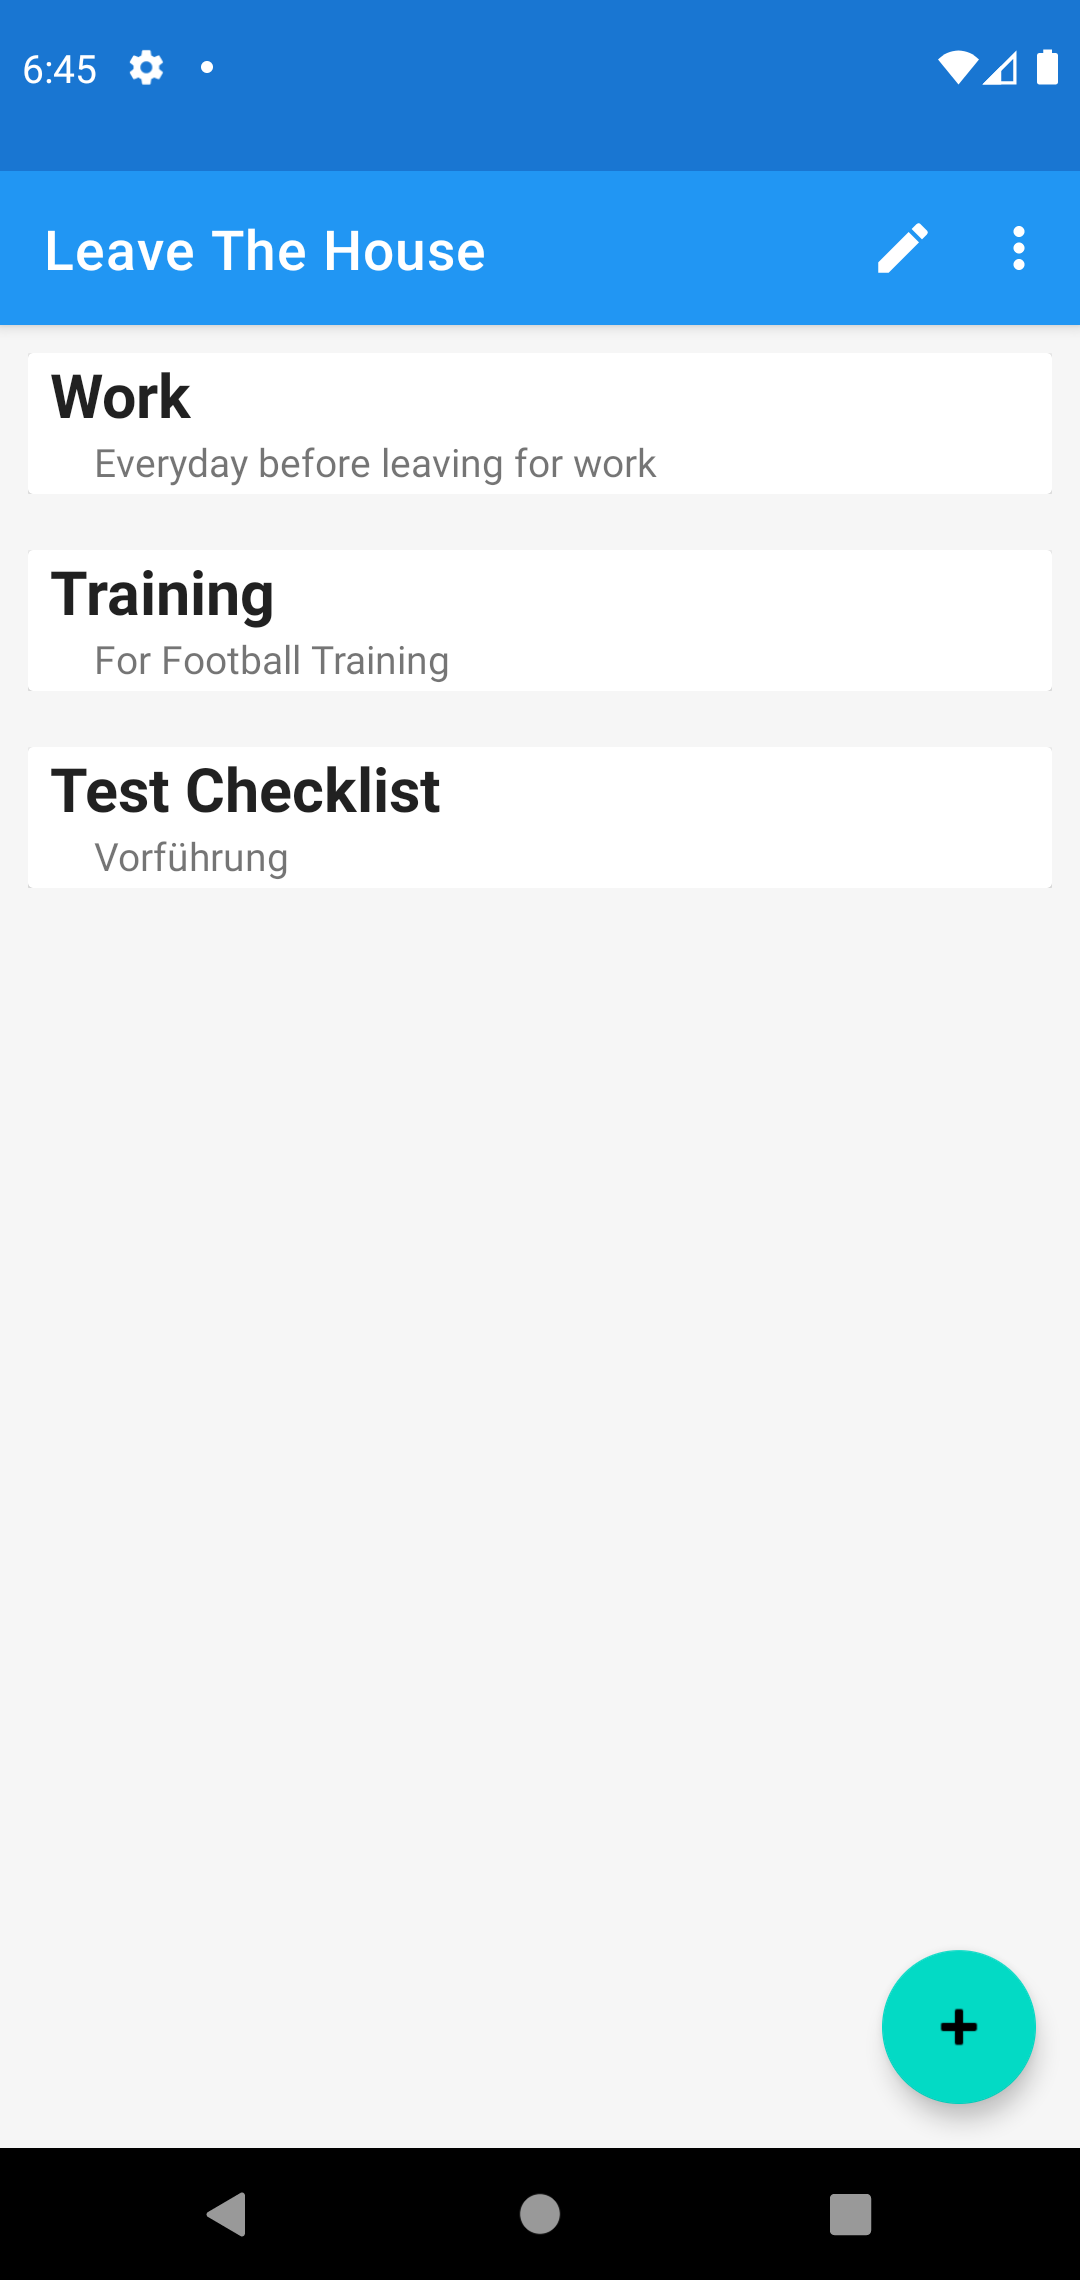
\includegraphics[width=.9\linewidth]{Bilder/MainActivity.png}
		\caption{MainActivity Ansicht}
		\label{fig:mainActivity}
	\end{minipage}
	\hfill
	\begin{minipage}{0.45\linewidth}
		\centering
		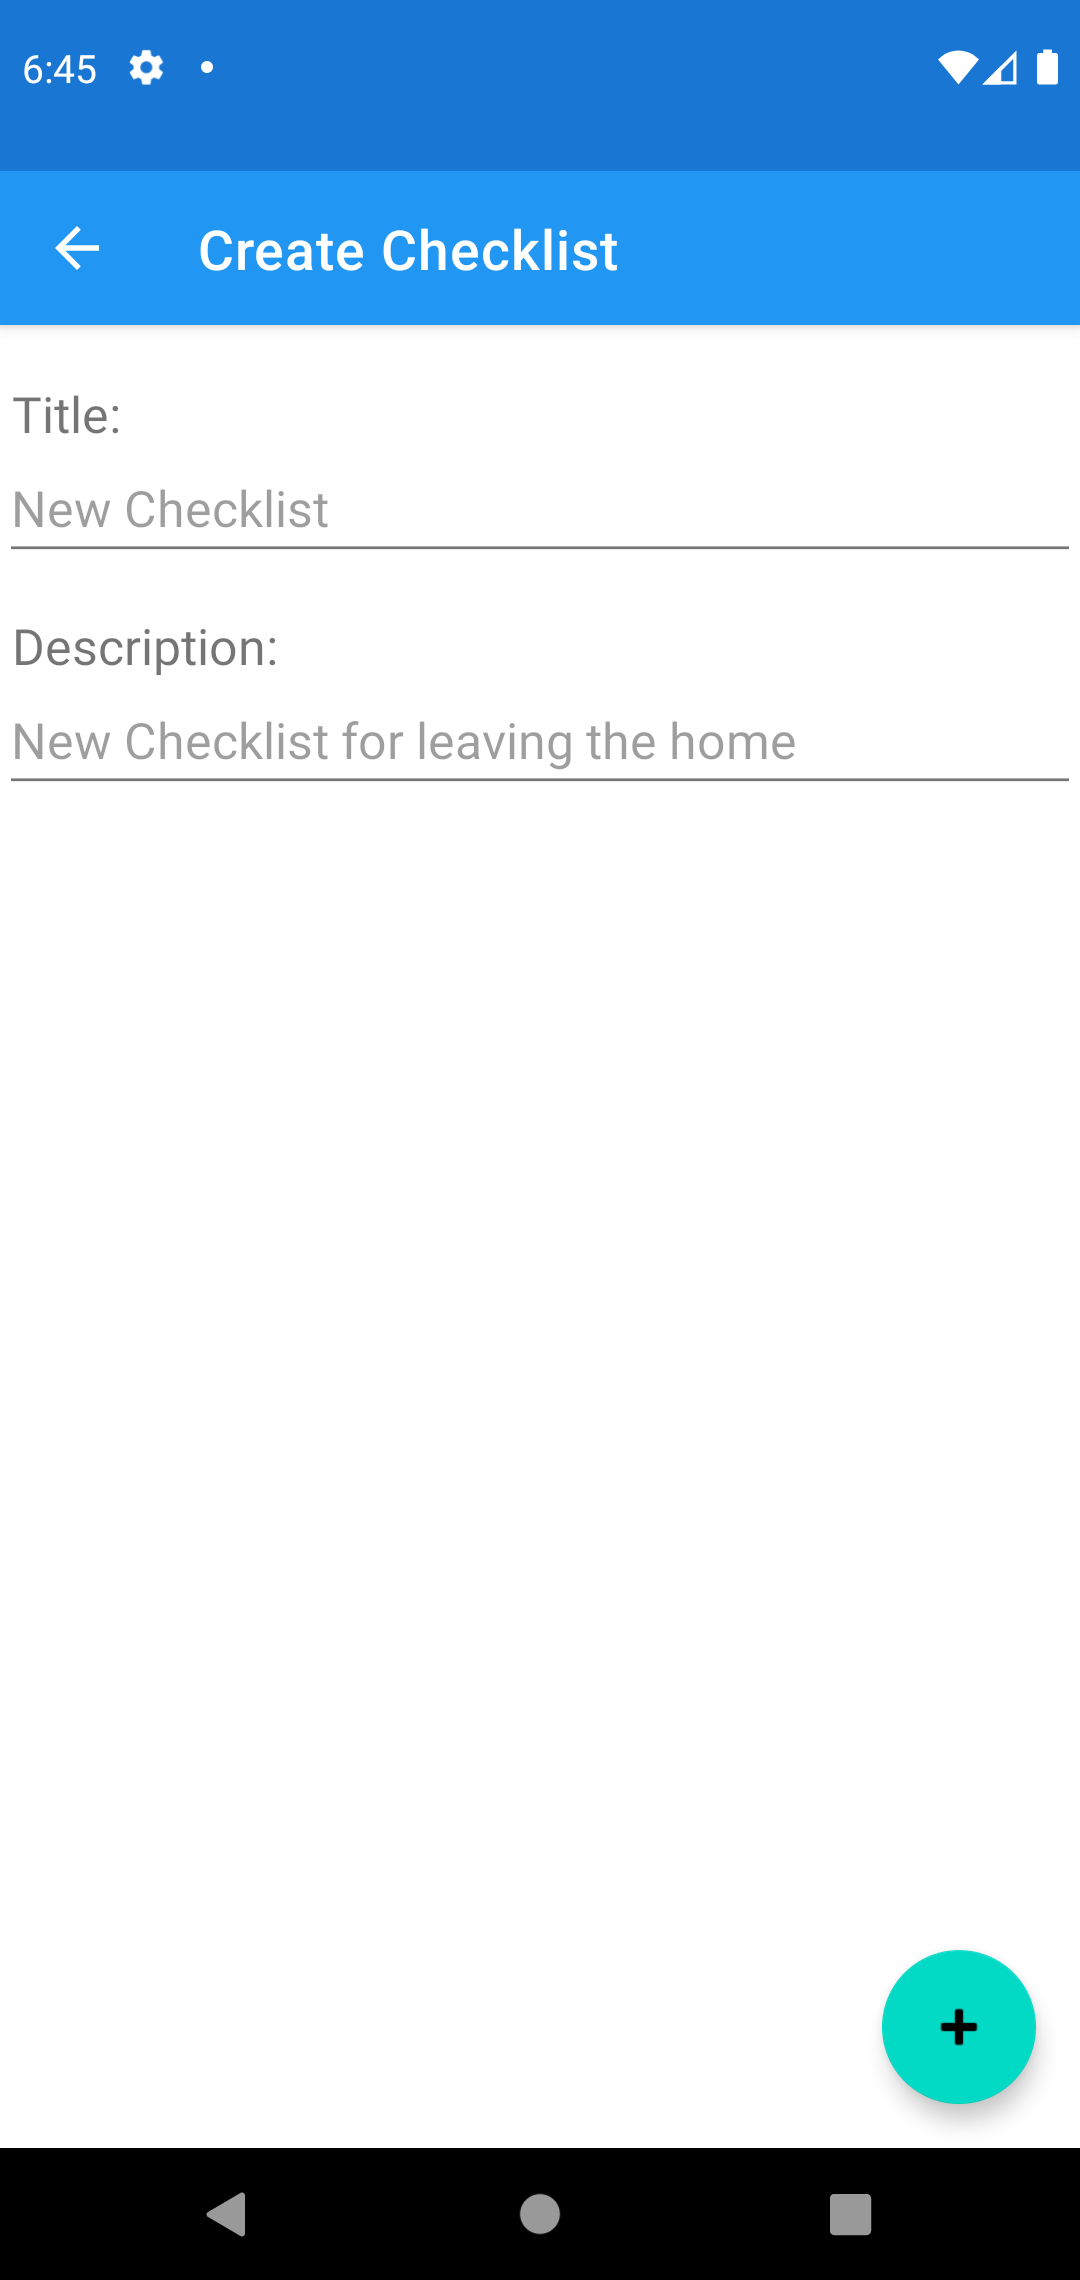
\includegraphics[width=.9\linewidth]{Bilder/CreateChecklist.png}
		\caption{CreateChecklist Ansicht}
		\label{fig:createChecklist}
	\end{minipage}
\end{figure}

Mit dem darstellen der erstellten Checkliste kann der erste Anwendungsfall, das erstellen einer Checkliste, nahezu als erfolgreich implementiert angesehen werden. Es ist dem Nutzer möglich über den Knopf die CreateChecklist Aktivität zu starten und seine Eingaben für Titel und Beschreibung zu tätigen. Durch bestätigen der Eingaben wird das neue Checklisten Objekt erstellt und dynamisch in der RecyclerView-Liste eingefügt und dargestellt. Der letzte fehlende Schritt ist das speichern und laden von erstellten Checklisten. Dieser Schritt wird in \autoref{subsec:speichereCheckliste} erläutert.

\subsection{Speichern von Checklisten}\label{subsec:speichereCheckliste}

Nachdem es dem Nutzer möglich ist Checklisten zu erstellen ist der nächste Schritt die erstellte Checkliste zu speichern und beim öffnen der App die gespeicherten Checklisten wieder zu laden und in der RecyclerView anzuzeigen.\\
Die erste Überlegung war hierfür ein Backend zu entwickeln, welches die Daten in einer Datenbank speichert und über eine \ac{API} ansprechbar ist. Voraussetzung für diese Herangehensweise wäre ein Nutzer-System. Jeder Nutzer müsste einen Account erstellen und diesen mit einem Passwort absichern. Ohne das könnten die gespeicherten Checklisten nicht dem richtigen Benutzer zugeordnet werden. Im verlauf der Entwicklung wurde sich gegen diese Herangehensweise entschieden und stattdessen das Speichern der Daten in einer Datei auf dem gerät gewählt. Grund dafür sind teilweise persönliche Präferenzen und Abwägung an den Vorteilen, die eine solche Lösung mit sich bringen würde. Auf der einen Seite würde es dem Nutzer ermöglichen Speicher auf dem Endgerät zu sparen. Auf der anderen Seite jedoch müsste ein Nutzer sich einen Account erstellen, bei dem er eine valide E-Mail Adresse, eventuell einen Nutzernamen und ein Passwort festlegen nur um Checklisten erstellen zu können. Zusätzlich müsste die Anwendung eine Internetverbindung haben und der Nutzer somit der App diesen Zugriff auf seinem gerät erlauben. Diese Punkte spiegeln auch die persönlichen Ablehnungen für diese Herangehensweise wieder, da ich dem erstellen von Accounts für skeptisch gegenüberstehe und dabei auch schon schlechte Erfahrungen mit Veröffentlichung von E-Mail Adressen nach Angriffen auf die Server gesammelt habe. Zudem sollte man für das erstellen und speichern einer Checkliste keine Internetverbindung brauchen, wobei dieser Punkt in der heutigen zeit zu vernachlässigen ist da jedes Endgerät, zumindest Zuhause per WLAN, eine Internetverbindung hat. Für diese App wurde sich jedoch für das lokale Speichern der Daten in einer Datei entschieden. Android unterstützt diese Herangehensweise durch das interne Datei System. Dies ermöglicht es Dateien Lokal auf dem Gerät persistent zu speichern. Als Format wurde hierfür die \ac{JSON} gewählt. Bei \ac{JSON} handelt es sich um ein Dateiformat, welches Programmiersprachen unabhängig und weit verbreitet ist. Die \ac{JSON}-Codierung ist zudem eine einfache Textform und lässt sich dadurch einfach zusammensetzten.\\
Das Speichern der Daten in der App erfolgt in einer dafür selbst geschriebenen Methode, um das Speichern unabhängig von einer spezifischen Standard Android Methode ausführen zu können. Diese Ansatz ermöglicht es die Speicher-Methode an den Stellen aufzurufen an denen es sinnvoll und notwendig ist. \autoref{code:saveChecklists} zeigt die geschriebene Methode und \autoref{code:checklistJSON} zeigt den Aufbau des \ac{JSON}-Format in dem die Checklisten gespeichert werden.
\\
\lstinputlisting[
label=code:saveChecklists,    % Label; genutzt für Referenzen auf dieses Code-Beispiel
caption=Methode zum Speichern von Checklisten,
captionpos=b,               % Position, an der die Caption angezeigt wird t(op) oder b(ottom)
style=EigenerKotlinStyle,     % Eigener Style der vor dem Dokument festgelegt wurde
firstline=1,                % Zeilennummer im Dokument welche als erste angezeigt wird
lastline=23                 % Letzte Zeile welche ins LaTeX Dokument übernommen wird
]{Quellcode/saveChecklists.kt}

\lstinputlisting[
label=code:checklistJSON,    % Label; genutzt für Referenzen auf dieses Code-Beispiel
caption=\ac{JSON} Format zum Speichern der Checklisten,
captionpos=b,               % Position, an der die Caption angezeigt wird t(op) oder b(ottom)
firstline=1,                % Zeilennummer im Dokument welche als erste angezeigt wird
lastline=10                 % Letzte Zeile welche ins LaTeX Dokument übernommen wird
]{Quellcode/ChecklistJSON.json}

Die Methode baut einen String im \ac{JSON}-Format. Dazu wird über die Liste der Checklisten iteriert und das Checklisten-Objekt in ein \ac{JSON}-Objekt konvertiert. Nach dieser Konvertierung wird das \ac{JSON}-Objekt in einen String umgewandelt und nach weiterer Formatierung mit dem gesamt String über String-Konkatenation zusammengeführt. Nachdem alle Checklisten formatiert und zu einem String geformt wurden muss dieser \glqq \ac{JSON}-String\grqq{} noch in einer Datei auf dem Gerät gespeichert werden. Dazu wird ein Datei-Objekt erstellt welches als Parameter das Lokale Dateiverzeichnis und den Dateinamen übergeben bekommt. Mithilfe eines Buffered- und eines FileWriters wird nun der String in die angegebene Datei in dem angegebene Verzeichnis geschrieben. Falls die Datei noch nicht existiert wird Sie erstellt und falls sie existiert wird der Inhalt überschrieben. Das überschreiben der vorhandene Datei ist vor allem für das Bearbeitern und Löschen für Checklisten relevant. Die Speichern-Methode wird an zwei Stellen in der MainActivity aufgerufen um zu gewährleisten, dass die Checklisten gespeichert werden. Diese zwei Stellen sind die Android-Methoden onStop() und onBackPressed(). Die onStop-Methode stammt vom Aktivitäten-Lebenszyklus und wird ausgeführt sobald die Aktivität in den Stopp-Status wechselt. Die onBackPressed-Methode erkennt wenn der Nutzer die Zurück-Taste auf dem Gerät betätigt um die Anwendung zu verlassen. Mithilfe dieser beiden Methoden sollte somit das Speichern der Checklisten gewährleistet sein.\\
Nachdem die Checklisten nun in einer lokalen Datei auf dem gerät gespeichert sind müssen diese Daten beim starten der App wieder eingelesen und dargestellt werden. Das Laden wird analog zu der Speichern-Methode in einer separaten Methode ausgeführt. Im Gegensatz zum Speichern wird hier zu Beginn der Methode mithilfe eines FileReaders und StringBuilders aus der \ac{JSON}-Datei wieder ein String im \ac{JSON}-Format erzeugt. Die einzelnen \ac{JSON}-Objekte werden dann aus dem String ausgelesen und aus den Daten ein Checklisten-Objekt erzeugt, welches der Checklisten-Liste hinzugefügt wird. Die Laden-Methode wird einmal in der onCreate-Methode der Main-Aktivität aufgerufen. Der Aufruf erfolgt vor dem erstellen des Adapter wodurch dieser zum Start der App die geladenen Daten darstellen kann ohne mit notifyDataSetChanged() ein neu generieren der RecyclerView Items anfragen zu müssen.\\
Mit diesen zwei Methoden kann der Anwendungsfall \glqq Checkliste erstellen\grqq{} als vollständig abgeschlossen angesehen werden. Der Nutzer kann nun Checklisten erstellen, welche sowohl direkt nach dem Erstellen als auch nach starten der App angezeigt werden.

\subsection{Erstellen von Aufgaben}\label{subsec:erstelleAufgaben}

Der zweite Anwendungsfall der im Verlauf der Entwicklung implementiert wurde ist das Erstellen von Aufgaben zu einer Checkliste. Hierzu soll der Nutzer auf eine Checkliste in der RecyclerView tippen können, um so diese Checkliste zu öffnen. Die Ansicht der geöffneten Checkliste soll dann die Möglichkeit bieten eine Aufgabe zu erstellen und diese ebenfalls in einer RecyclerView-Liste anzuzeigen.\\
Der erste Schritt ist das dynamische öffnen des an getippten Checklisten-Listenelement. Dazu wird der ChecklistViewHolder um eine Vererbung von der OnClickListener-Klasse erweitert. Dadurch kann die onClick-Methode innerhalb des ViewHolder überschreiben und mit eigenen Methodenaufrufen ausgestattet werden. Durch die generelle Funktionsweise des Adapter und ViewHolder ist somit jedes Listenelement mit dieser Funktion ausgestattet und kann auf die Interaktion des Nutzer reagieren. Für das öffnen der Checkliste wurde die neue Aktivität OpenChecklistActivity erstellt. Der Layout-Aufbau gleicht dem der MainActivity. Es besteht ebenfalls aus einer Werkzeugleiste, einer RecyclerView und einem Knopf in der unteren rechten Ecke. Im Gegensatz zur MainActivity steht jedoch nicht der Name der App sondern der Titel der geöffneten Checkliste als Titel in der Werkzeugleiste. Dies ermöglicht es dem Nutzer zu erkennen welche Checkliste er aktuell geöffnet hat. Innerhalb der onClick-Methode wird die OpenChecklistActivity durch einen Aufruf von startActivity gestartet. Das Layout kann in \autoref{fig:taskView} eingesehen werden. Der Knopf unten rechts erfüllt die gleiche Aufgabe wie sein äquivalent in der MainActivity. Mit ihm wird die CreateTask Aktivität gestartet in der der Nutzer der Aufgabe einen Titel und eine Beschreibung geben kann (vgl. \autoref{fig:createTask}). Diese werden wieder in der onActivityResult-Methode ausgewertet und ein neues Aufgaben Objekt damit erstellt. Die Aufgaben werden dann mithilfe eines TaskRecyclerViewAdapter und der darin erstellten Klasse TaskViewHolder in der RecyclerView dargestellt. Der letzte fehlende Schritt ist das Speichern und Laden der Aufgaben zu der jeweiligen Checkliste. An dieser Stelle ist ein Problem mit dieser Umsetzung aufgetreten. Die Aufgaben wurden in der openChecklistAktivität erstellt und wie die Checklisten in der MainActivity in einer ArrayList gehalten. Die Speichermethode befindet sich jedoch in der MainActivity da nur dort eine Liste mit allen Checklisten vorhanden ist. Es gibt jedoch keine Möglichkeit die Aufgabenliste über den Adapter an die MainActivity zu geben. Wie dieses Problem gelöst werden konnte wird im \autoref{sec:problem} erläutert.
\\
\begin{figure}[h]
	\centering
	\begin{minipage}{0.45\linewidth}
		\centering
		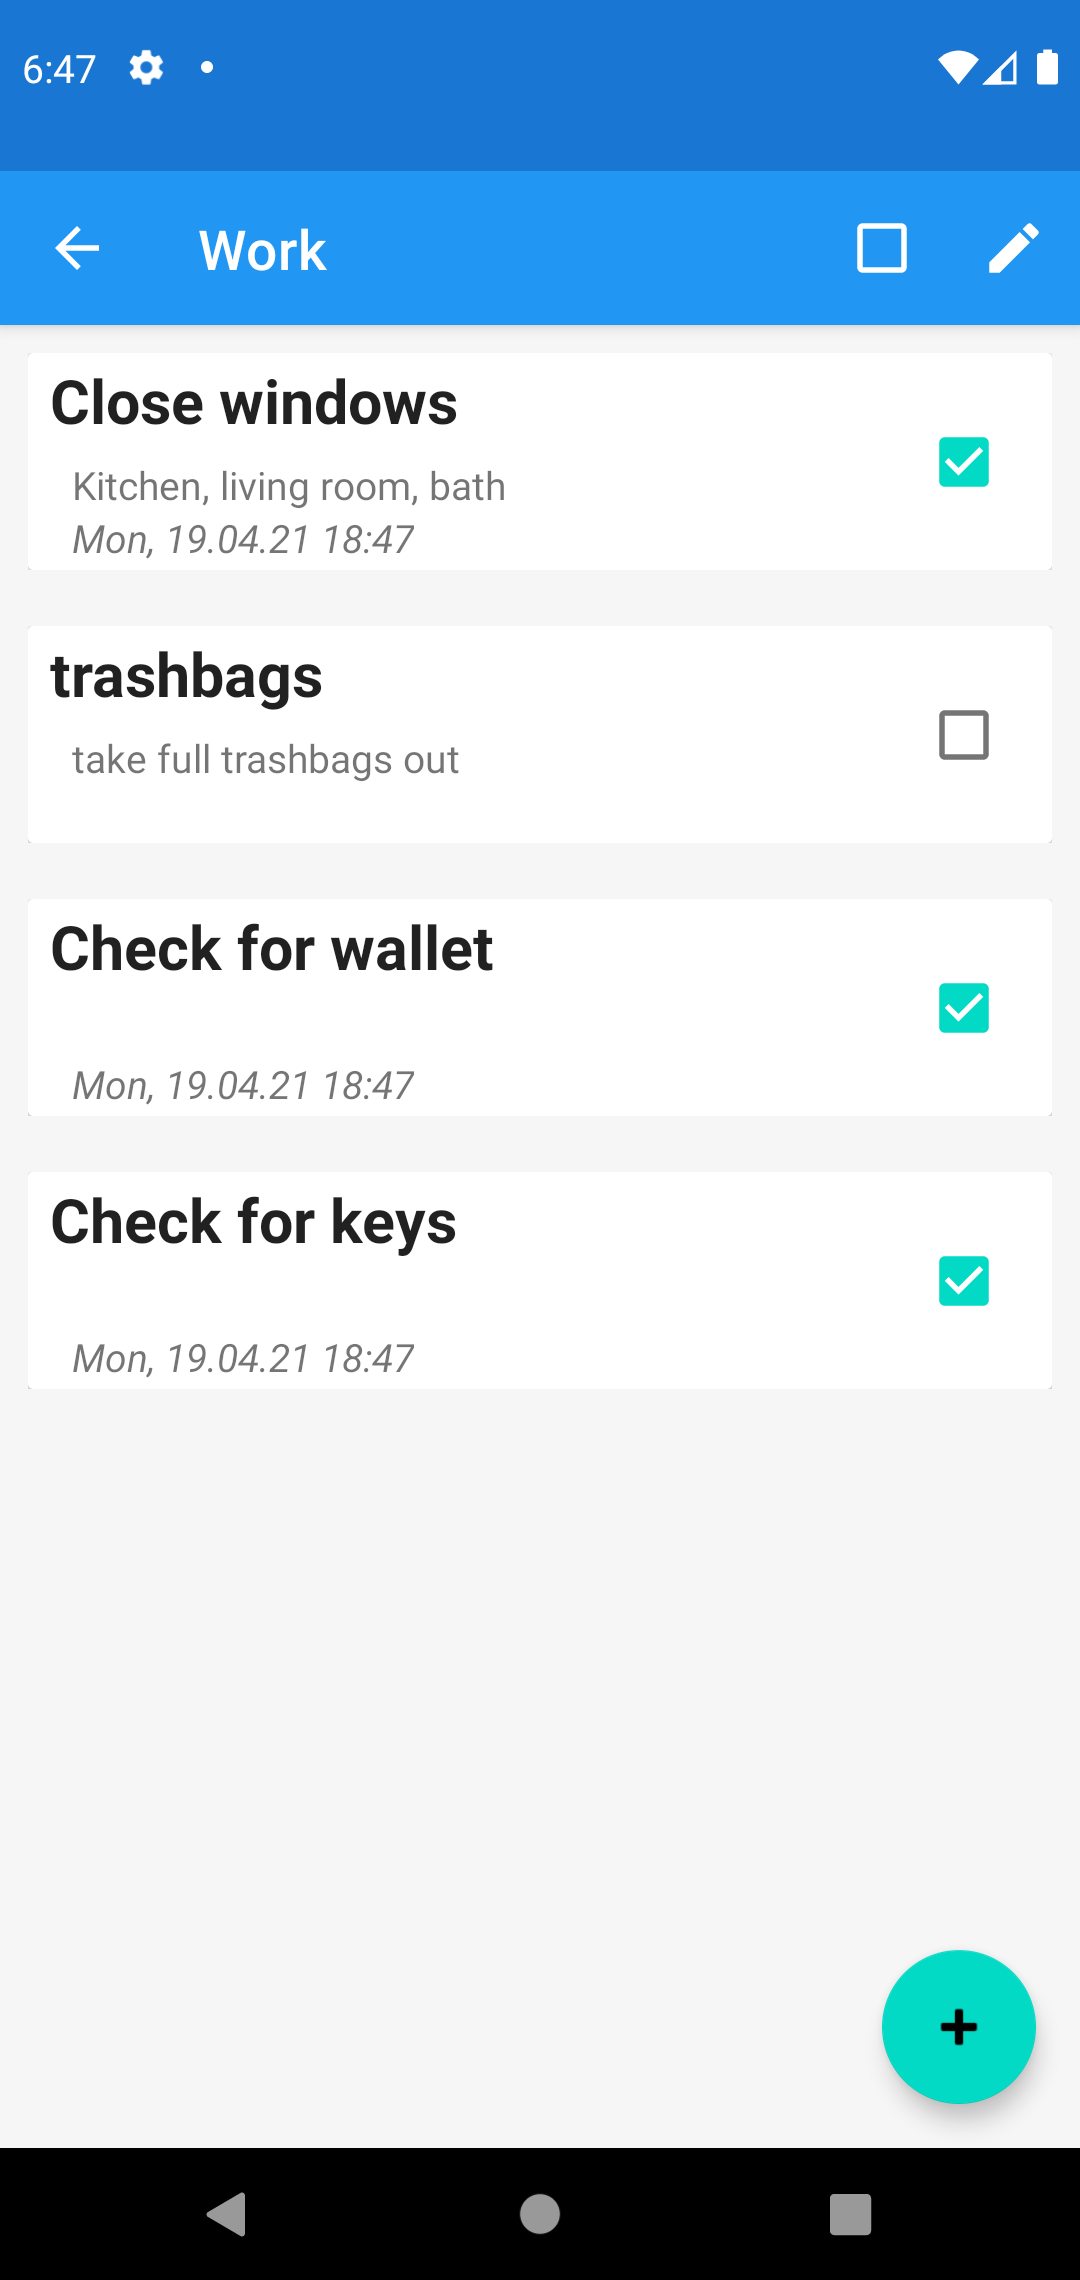
\includegraphics[width=.9\linewidth]{Bilder/TaskView.png}
		\caption{Ansicht einer geöffneten Checkliste}
		\label{fig:taskView}
	\end{minipage}
	\hfill
	\begin{minipage}{0.45\linewidth}
		\centering
		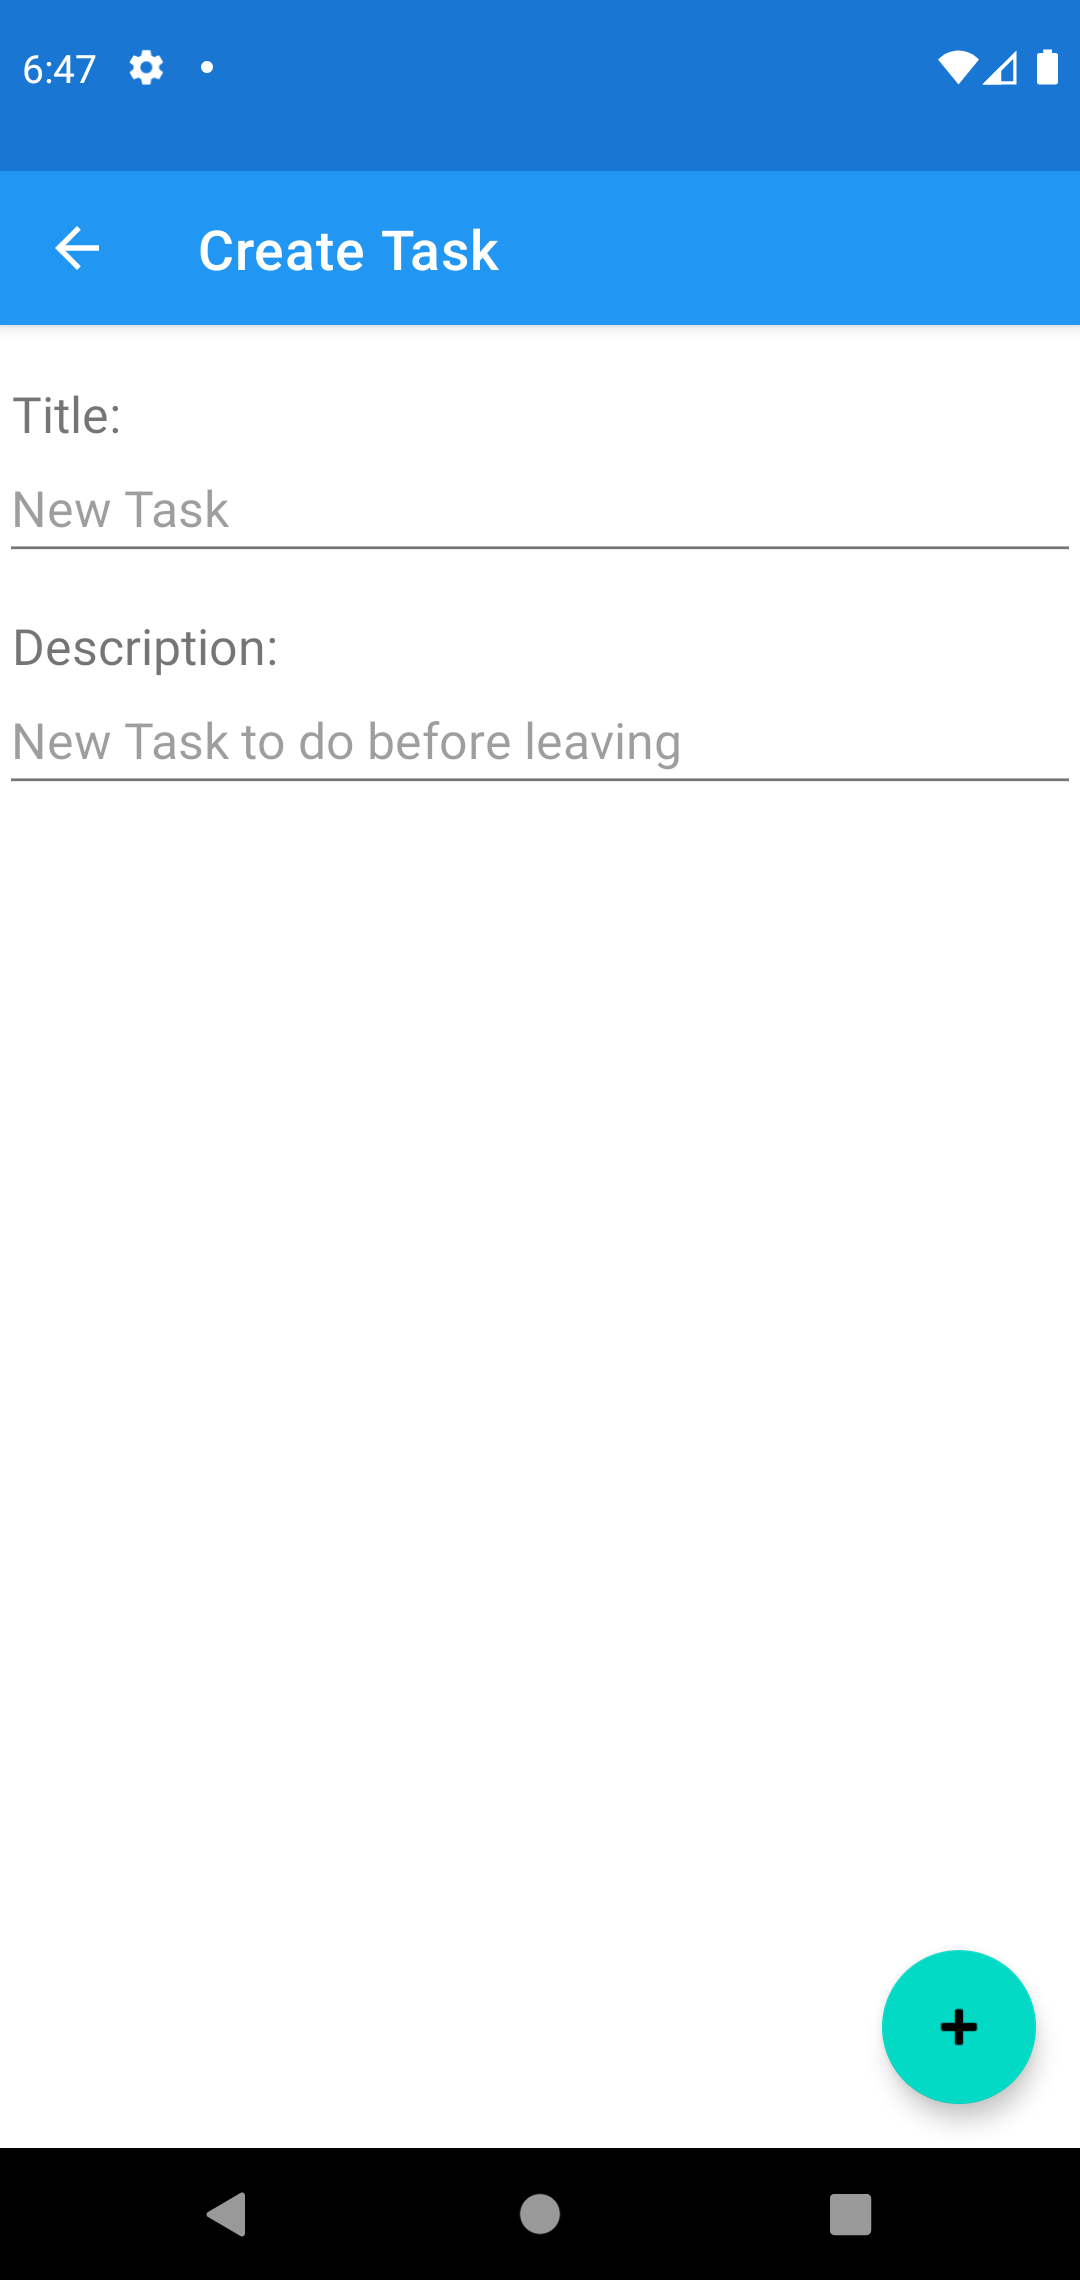
\includegraphics[width=.9\linewidth]{Bilder/CreateTask.png}
		\caption{CreateTask Ansicht}
		\label{fig:createTask}
	\end{minipage}
\end{figure}

Nach der Lösung des Problems fehlt noch das Speichern und Laden der Aufgaben. Dazu wurden die dafür geschriebenen Methoden angepasst. Der angepasste Code kann in \autoref{code:saveAll} eingesehen werden. Um die Aufgaben zu Speichern wird ein \ac{JSON}Array-Objekt erstellt. Jede Aufgabe wird dann, wie die Checklisten auch, in ein \ac{JSON}-Objekt umgewandelt und an den \ac{JSON}Array angehängt. Nachdem alle Aufgaben als \ac{JSON}-Objekte an den \ac{JSON}Array angehängt wurde wird dieser dem \ac{JSON}-Objekt der Checkliste beigefügt. Der Rest der Methode bleibt unverändert. Im Anschluss an die Erstellung des \ac{JSON}-String wird über den FileWriter die \ac{JSON}-Datei geschrieben und auf dem Gerät im lokalen Speicher gesichert. Das neue resultierende \ac{JSON}-Format wird in \autoref{code:saveAll} beispielhaft gezeigt.
\\
\lstinputlisting[
label=code:saveAll,    % Label; genutzt für Referenzen auf dieses Code-Beispiel
caption=Methode zum Speichern von Checklisten und Aufgaben,
captionpos=b,               % Position, an der die Caption angezeigt wird t(op) oder b(ottom)
style=EigenerKotlinStyle,     % Eigener Style der vor dem Dokument festgelegt wurde
firstline=3,                % Zeilennummer im Dokument welche als erste angezeigt wird
lastline=25                 % Letzte Zeile welche ins LaTeX Dokument übernommen wird
]{Quellcode/saveAll.kt}

\lstinputlisting[
label=code:allJSON,    % Label; genutzt für Referenzen auf dieses Code-Beispiel
caption=\ac{JSON} Format zum Speichern der Checklisten und Aufgaben,
captionpos=b,               % Position, an der die Caption angezeigt wird t(op) oder b(ottom)
firstline=1,                % Zeilennummer im Dokument welche als erste angezeigt wird
lastline=23                 % Letzte Zeile welche ins LaTeX Dokument übernommen wird
]{Quellcode/AllJSON.json}

Mit diesen Änderungen ist der Anwendungsfall Aufgabe erstellen abgeschlossen. Während der Entwicklung des Anwendungsfall wurde zugleich der Anwendungsfall des abhacken von Aufgaben implementiert. Hierzu wurde der TaskViewHolder, gleich wie der ChecklistViewHolder, um einen onClickListener erweitert. Darin wird eine Methode aufgerufen die Abhängig vom aktuellen Status in den jeweils anderen gewechselt. Hier wird jetzt ein Unterschied des Layout eines Aufgaben-Listenelement zum bereits erläuterten Checklisten-Listenelement deutlich. Dieses hat neben dem Titel- und Beschreibungstextfeld zusätzlich eine Checkbox auf der rechten Seite. Über diese Checkbox wird der aktuelle Staus der Aufgabe repräsentiert. Eine abgehackte Checkbox gilt als erledigt, eine leere als offen. In \autoref{fig:taskView} sind die Checkbox so wie die beiden möglichen Zustände deutlich zu erkennen. In der onClick-Methode wird neben dem Wert des Aufgaben-Objekt auch der Wert der Checkbox im jeweiligen Layout des an getippten ViewHolder-Elements gewechselt.\\
Durch diese kleine Ergänzung am Layout der Aufgaben und dem ViewHolder kann auch dieser Anwendungsfall als erfolgreich implementiert angesehen werden.

\subsection{Bearbeiten von Checklisten und Aufgaben}\label{subsec:bearbeiten}

Als nächstes wurden die Anwendungsfälle des Bearbeiten einer Checkliste und einer Aufgabe implementiert. Die Idee hierbei ist den gleichen Ablauf für Checklisten und Aufgaben zu verwenden, wie es auch beim Erstellen der Fall ist. Das Erstellen läuft in beiden Fällen über den Knopf in der rechten unteren Ecke der nahezu identische Aktivitäten für die Benutzereingaben öffnet. Die Wahl die Abläufe gleich zu implementieren lässt sich auf \ac{UX}, zu deutsch Nutzererfahrung zurückführen. Wenn gleiche Funktionen innerhalb einer Anwendung an verschiedenen Stellen zu finden sind löst dies bei einem Benutzer Unbehagen aus. Durch verwenden einer Funktion versteht der Nutzer den Ablauf. Versucht er nun eine gleiche Funktion an einer anderen Stelle der gleichen Anwendung durchzuführen wird er Versuchen auf seine Erfahrung des vorherigen Ablauf zurückzugreifen. Das beruht auf dem grundlegenden Verständnis dass gleiche Funktionen den gleichen Ablauf haben sollte. Ein gutes Beispiel hierfür ist das sogenannte Norman-Tür Prinzip. Bei einer Norman-Türe handelt es sich um jede Türe deren Benutzung verwirrend oder schwierig ist. Türen haben an sich einen einfach Anwendungsfall der sich in der Durchführung lediglich durch den Türgriff unterscheidet. Im Lauf seines Lebens lernt man das eine Tür mit Griff aufgezogen wird, während man eine Tür die nur eine Platte als Griff hat eher drückt. Sobald man durch eine Tür hindurch will wendet man automatisch dieses gesammelte Verständnis an um die Tür zu öffnen. An dieser Stelle tritt die Norman-Tür in Kraft. Kann man nicht ausmachen wie oder wo die Tür geöffnet hat scheitert diese Tür an dem simplen und einzigen Anwendungsfall jeder Tür. Der Nutzer sollte nicht erst zweimal überlegen, suchen oder ein Schild lesen müssen um zu wissen wie die Tür funktioniert. Es ist einfach nur eine Tür. Jede Tür die nicht intuitiv richtig geöffnet werden kann ist eine Norman-Tür. Sie führt beim Nutzer zur Verwirrung oder mitunter zur Verzweiflung und Selbstschuld. Doch der Nutzer ist in keinem Fall selbst Schuld. Die Tür legt die Annahme die der Nutzer zur Nutzung trifft durch das Design fest. Die gleiche verwirrte und verzweifelte Reaktion des Nutzer kann auch in der Softwareentwicklung auftreten. Durch die Benutzung der Anwendung bauen Nutzer ein Mentales Modell auf wie sie diese App zu bedienen haben. Daraus entstehen wieder Annahmen und Vermutungen wie bestimmte Anwendungsfälle durchzuführen sind, vergleichbar mit dem öffnen der Tür. Kann der Nutzer also nicht eine Aufgabe auf die Selbe weise wie Checkliste erstellen obwohl sich das Layout gleicht treten beim Nutzer zweifel an seinem Mentalen Modell und Verständnis über die App auf. Dies kann beim Nutzer zu Verwirrung führen was in einer schlechten Nutzererfahrung mündet. Anwendungen die eine schlechte Nutzererfahrung hervorrufen werden nicht so gern verwendet wie vergleichbare Anwendungen mit guter Nutzererfahrung. Aus diesen Gründen wurde bei der Entwicklung Weert darauf gelegt Anwendungsfälle welche die gleiche Funktion für Checklisten und Aufgaben erfüllen so ähnlich wie möglich zu implementieren. Dies soll zu einer guten Nutzererfahrung und einem einfachen Mentalen Modell zu Benutzung dieser App führen.\footnote{Interaktive Systeme Vorlesung}\\
Da, wie nun deutlich gemacht wurde, die Implementierung zum Bearbeiten für Checklisten und Aufgaben identisch ist wird der Vorgang nur einmal erläutert. Um Checklisten oder Aufgaben zu bearbeiten wird ein Bearbeitungsmodus eingeführt. Dieser kann durch Betätigen eines Knopfes in der Werkzeugleiste ein und ausgeschaltet werden (vgl. \autoref{fig:mainActivity} und \autoref{fig:taskView}). Der Knopf wird durch das Bearbeitungssymbol eines Bleistift dargestellt. Dieser soll klarmachen was dieser Knopf bewirkt. Im nächsten Schritt wird sich die Lösung des Aufgaben speichern Problems zunutze gemacht und um eine Funktion erweitert. Durch tippen auf einen RecyclerView-Listeneintrag mit Aktiviertem Bearbeitungsmodus öffnet sich nun eine Aktivität zum Bearbeiten des Eintrags. Hierbei wird sich auch einer Eigenschaft des Layouts zum erstellen eines Eintrags bedient. Die Text- und Eingabefelder befinden sich nicht fest in dem Layout dieser Aktivität. Sie sind in einer weiteren XML-Datei beinhaltet und werden über den Include-Tag in das Layout dieser Aktivität eingebunden. Dies ist sowohl bei den Checklisten als auch den Aufgaben der Fall. Für das Bearbeiten wurden lediglich neue Aktivitäten mit dem Layout einer Werkzeugleiste, dem einbinden der Text- und Eingabefelder und einem neuen Bestätigungsknopf in der unteren rechten Ecke angelegt. Beim öffnen der Bearbeitungsaktivitäten werden die aktuellen Daten in den Eingabefeldern als Text gesetzt, sodass der Nutzer diese \zB im Falle eines Tippfehlers einfach beheben kann. Mit bestätigen der Änderungen über den Knopf werden die Daten des gedrückten Elements angepasst. Da die Datei beim speichern komplett neu geschrieben wird sind für das Speichern keine Änderungen nötig. Das Layout kann in \autoref{fig:editView} eingesehen werden.\\
Somit können nun auch die Anwendungsfälle zum Bearbeiten als abgeschlossen angesehen werden.

\subsection{Löschen von Checklisten und Aufgaben}\label{subsec:löschen}

Nach dem Bearbeiten soll es dem Nutzer auch möglich gemacht werden Checklisten und Aufgaben zu löschen. Auch bei diesen Anwendungsfällen wird auf die Nutzererfahrung geachtet. Auf diese wurde genauer in \autoref{subsec:bearbeiten} eingegangen. Wie beim Bearbeiten auch wird der Anwendungsfall nur einmal beschreiben, da er für Checklisten und Aufgaben identisch ist. Um eine Checkliste Löschen zu können muss der Anwender den Bearbeitungsmodus aktivieren und auf das zu löschende Listenelement tippen. Dadurch öffnet sich die Bearbeitungsaktivität. Wie bereits beschrieben hat diese ebenfalls eine Werkzeugleiste. Dieser wird ein Knopf mit dem Symbol eines Mülleimers hinzugefügt. Nach betätigen des Löschen Knopfes öffnet sich ein Dialogfenster in dem das Löschen des Listenelement bestätigt werden muss. Der Dialog soll das Löschen eines Elements durch versehentliches antippen des Knopfes verhindern. Es wurde jeweils eine Dialog Klasse für Checklisten und Aufgaben angelegt. Diese Klassen erben von der Klasse AppCompatDialogFragment(). Ein Fragment ist ähnlich wie die Aktivität ein Grundlegendes Element von Android. Es handelt sich dabei um einen Teil der Nutzeroberfläche. Fragmente haben ihr eigenes Layout, eigenen Lebenszyklus und kann selbst Nutzereingaben verarbeiten. Fragmente können jedoch nicht eigenständig existieren sondern müssen von einer Aktivität oder einem anderen Fragment gehalten werden. Sie stellen dann einen Teil der Ansicht der Aktivität dar. Um den Dialog zu öffnen wird eine Instanz der erstellten Dialog-Klasse erstellt und über den $.show$ Befehl geöffnet. In der Dialog-Klasse wird, wie auch bei Aktivitäten, eine onCreate-Methode überschrieben. Im Gegensatz zu Aktivitäten wird hier nicht das Layout gesetzt sondern in diesem Fall über einen AlertDialogBuilder gebaut. Dem Builder werden Titel, Text und jeweils ein positiver und negativer Knopf mit Text als Komponenten mitgegeben. Der resultierende Dialog wird in \autoref{fig:deleteDialog} dargestellt. In der Aktivität die den Dialog erstellt hat wird über eine Methode die Antwort des Nutzers übergeben und die Aktivität im Falle einer Bestätigung beendet. Die Einträge werden gelöscht indem der getippte Listeneintrag aus der jeweiligen Datenliste des Adapter entfernt wird. Identisch zum bearbeiten ist ebenfalls keine Änderung bei der Speichern Funktion notwendig, da beim schreiben der Datei nur die Einträge der Datenliste gespeichert werden.\\
Mit der Implementation des Löschen sind alle Grundlegenden im Umfang definierten Anwendungsfälle für die erstellten Klassen vorhanden. Der letzte Anwendungsfall, das entfernen aller Haken, stellt eine Zusatzfunktion für eine Bessere Nutzererfahrung dar und wird in \autoref{subsec:Haken} erläutert.
\\
\begin{figure}[h]
	\centering
	\begin{minipage}{0.45\linewidth}
		\centering
		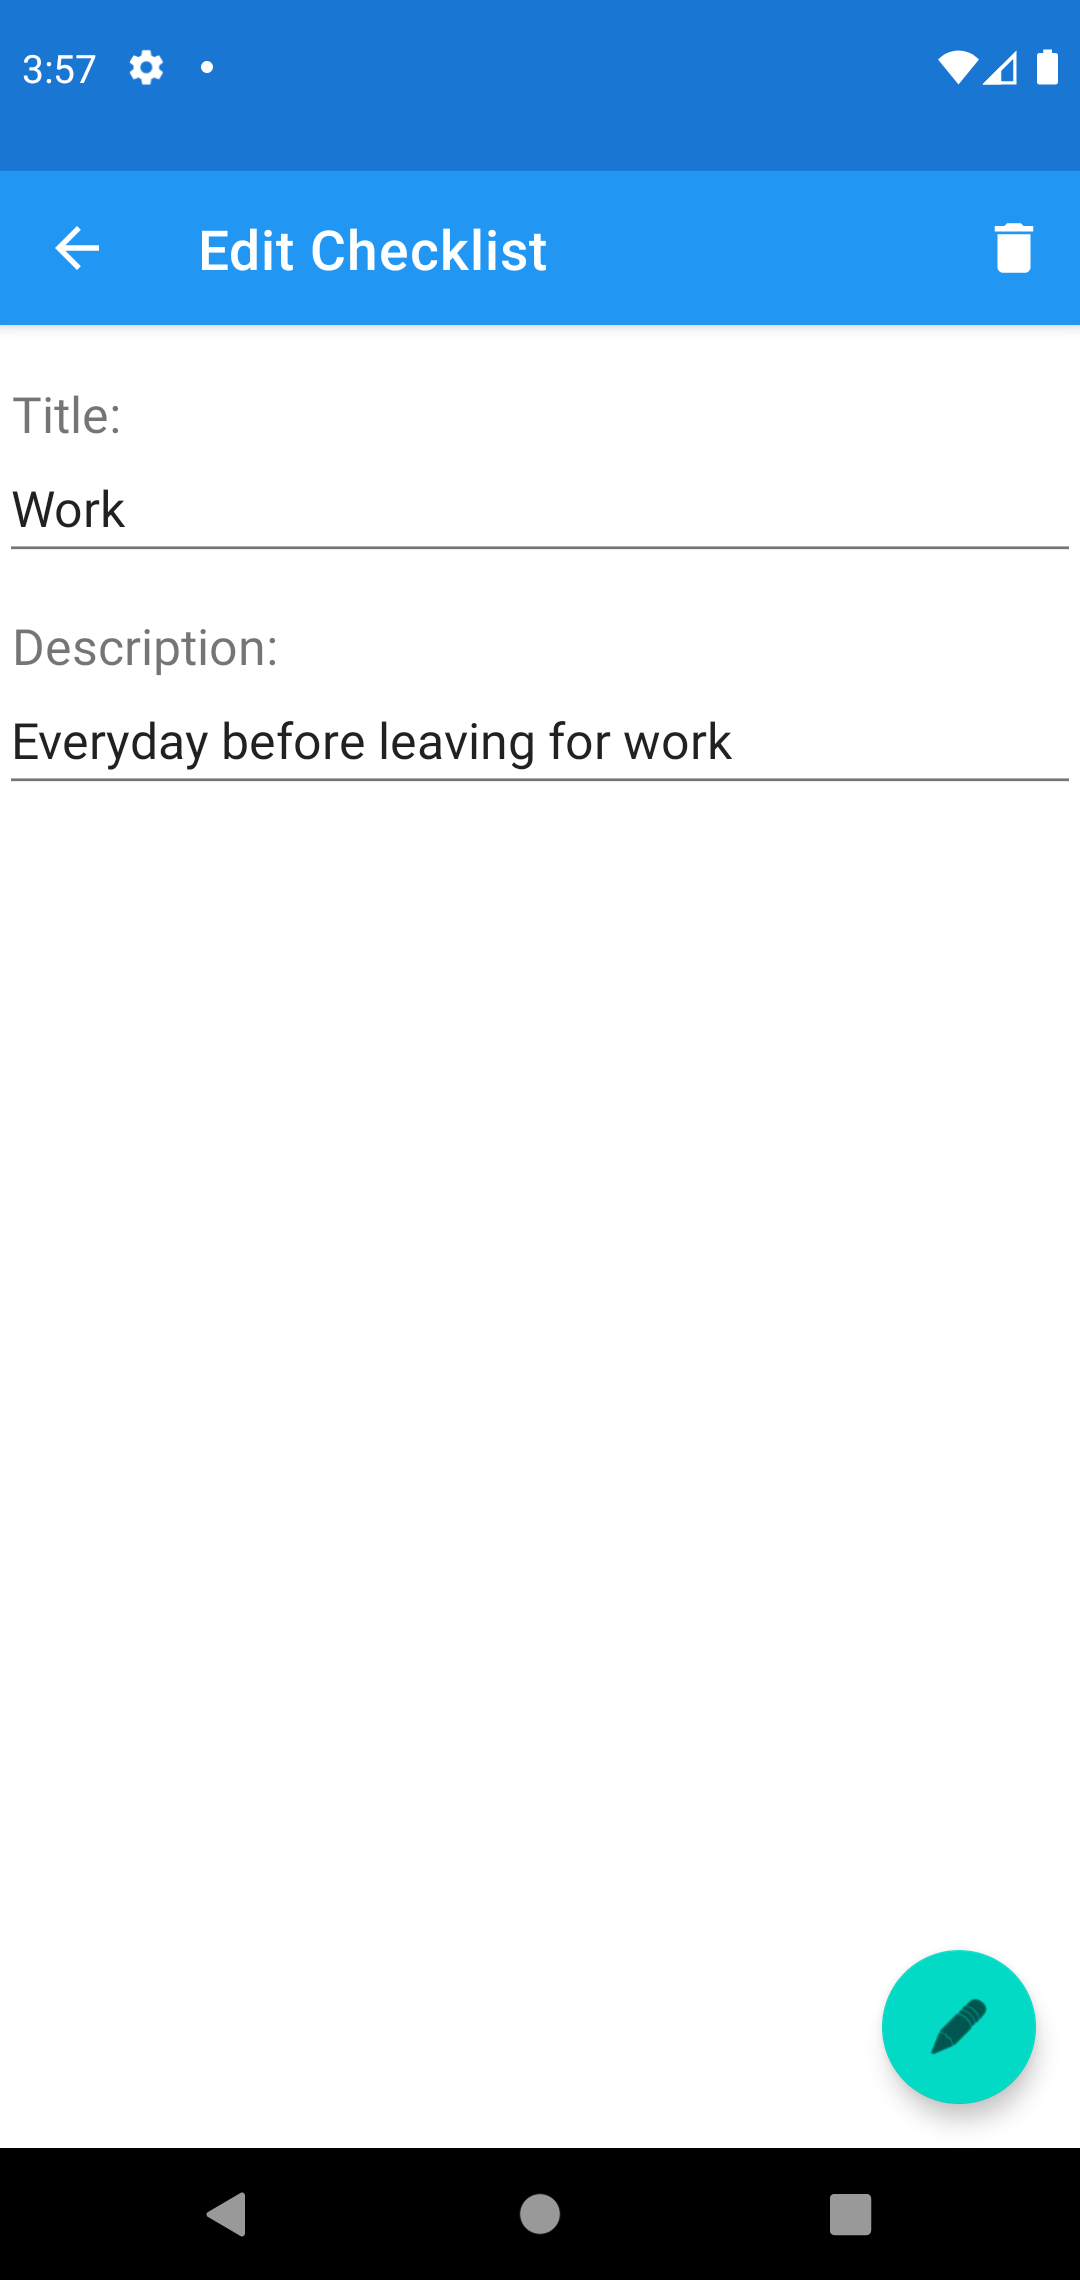
\includegraphics[width=.9\linewidth]{Bilder/EditChecklist.png}
		\caption{Ansicht zum Bearbeiten Checkliste}
		\label{fig:editView}
	\end{minipage}
	\hfill
	\begin{minipage}{0.45\linewidth}
		\centering
		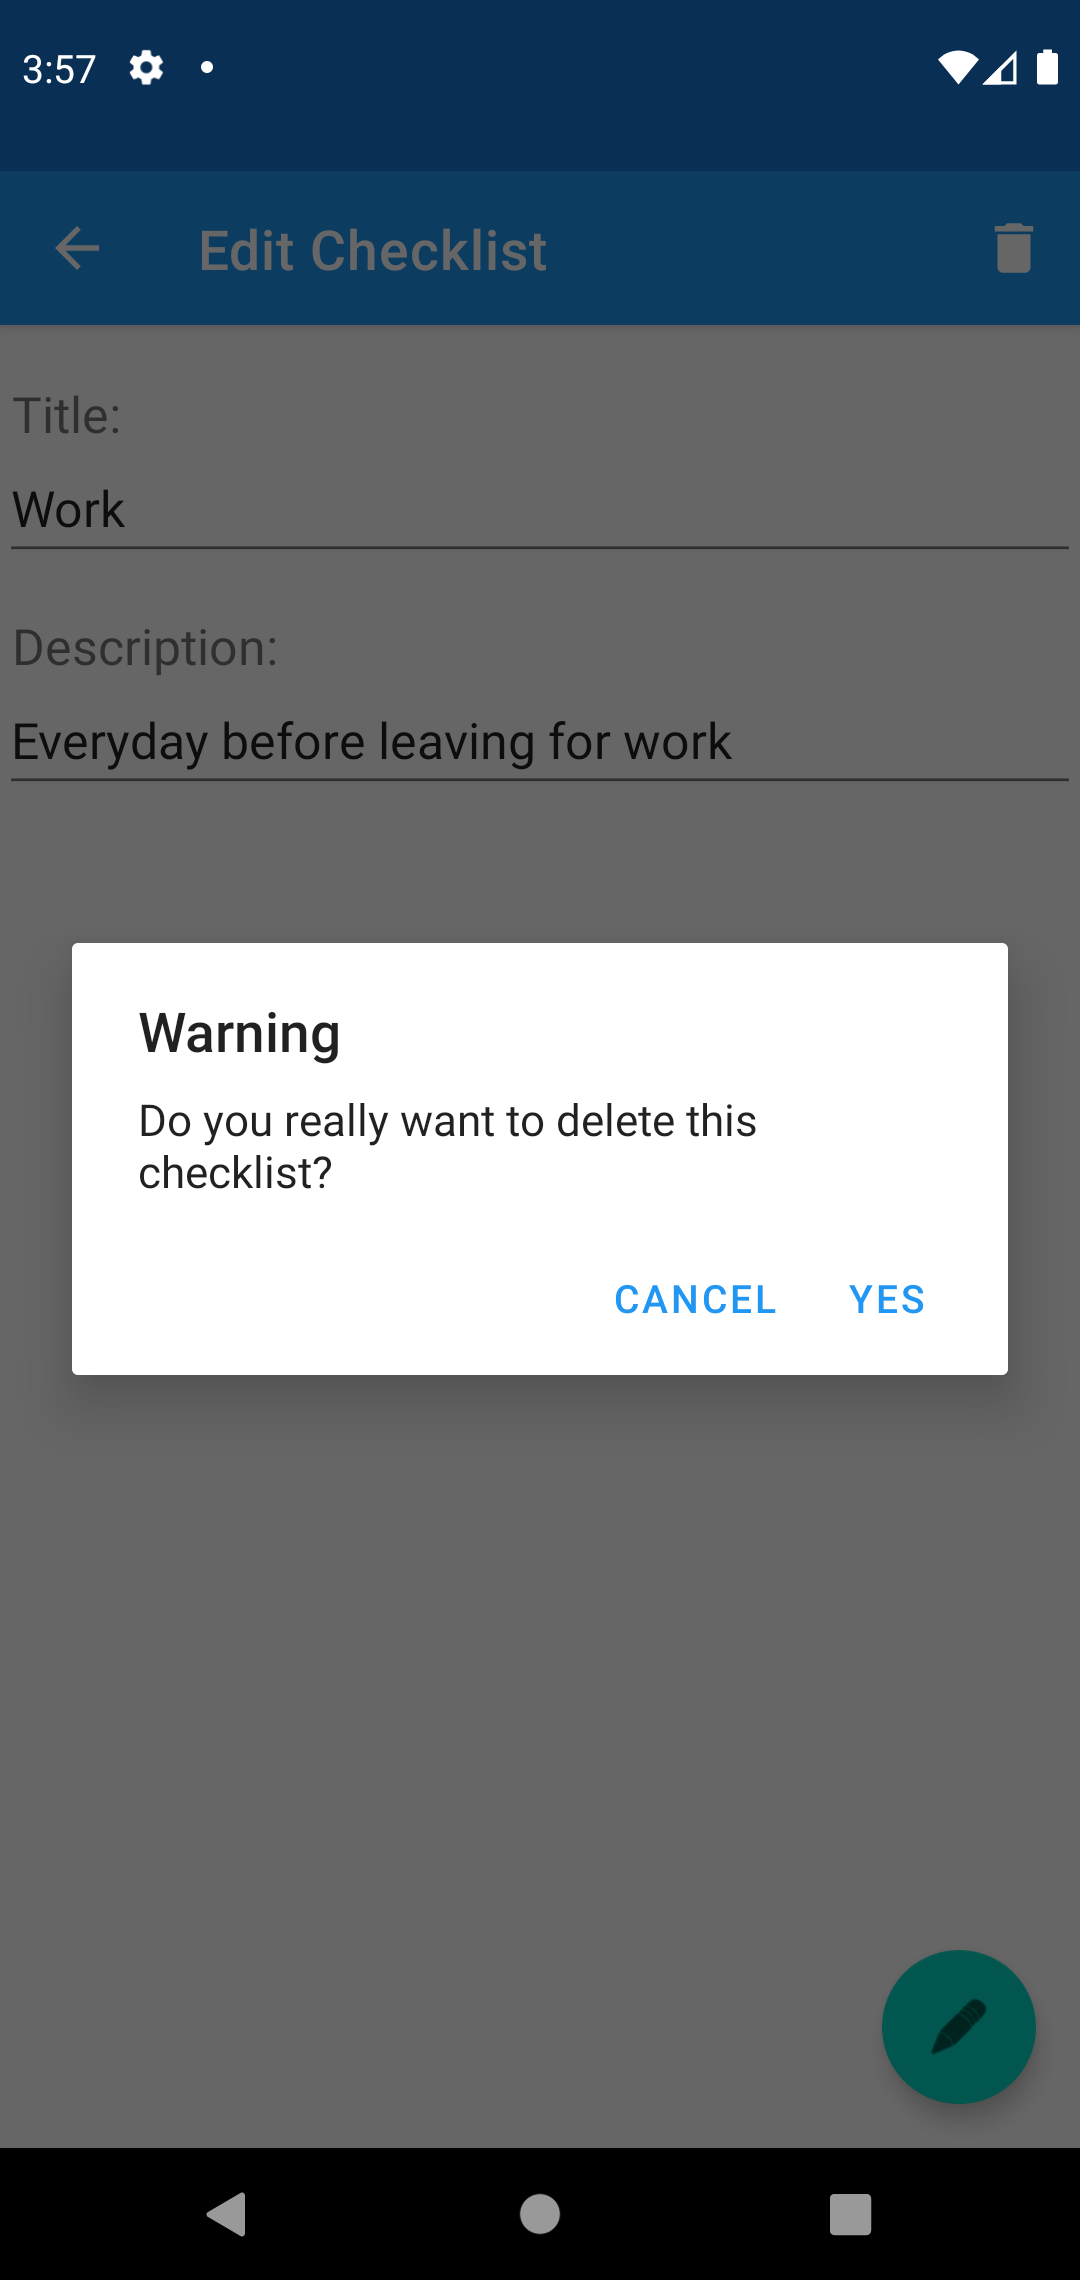
\includegraphics[width=.9\linewidth]{Bilder/DeleteChecklist.png}
		\caption{Dialog beim Löschen einer Checkliste}
		\label{fig:deleteDialog}
	\end{minipage}
\end{figure}

\subsection{All Haken entfernen}\label{subsec:Haken}
Die Idee hinter dieser Anwendung beruht auf dem täglichen Nutzen beim verlassen des Hauses oder Arbeitsplatzes. Je nach Umfang kann eine Checkliste unter Umständen relativ viele Aufgaben beinhalten. Mit dem derzeitigen Funktionsumfang müsste der Nutzer bei jeder erneuten Nutzung einer Checkliste die Haken einzeln von jeder Aufgabe entfernen, was sich als aufwendig herausstellen kann. Aus diesem Grund wurde der Anwendungsfall \glqq Alle Haken entfernen\grqq{} implementiert. Für diese Funktion wurde die Werkzeugleiste in der Aufgabenansicht um einen Knopf erweitert. Der Knopf kann bereits auf \autoref{fig:taskView} links des Bearbeiten-Knopfes gesehen werden. Durch betätigen dieses Knopfes werden alle Checkboxen und die Attribute der Aufgaben, welche des Status halten, auf nicht abgehackt gesetzt.\\
Mit der Implementation dieses Anwendungsfall sind alle in der Projektdefinition geplanten Anwendungsfälle implementiert und die App hat ihren grundlegenden Status erreicht. Die Funktionalität der einzelnen Anwendungsfälle wird in \autoref{sec:tests} mithilfe von Espresso- und Nutzer-Tests getestet. Die Entwicklung gilt jedoch hiermit als, für diesen Teil, abgeschlossen.

\subsection{Erweiterung}\label{subsec:erweiterung}
Wie bereits in \autoref{sec:umfang} und \autoref{sec:risiko} erläutert sind nach Rücksprache mit dem Betreuer Ideen für weitere Anwendungsfälle aufgetreten. Im Umfang dieser Studienarbeit wurde einer dieser neuen Anwendungsfälle in die Anwendung implementiert. Dabei handelt es sich um den Zeitstempel an den Aufgaben. Dieser soll verdeutlichen ob der Hacken an einer Aufgabe noch von einem Vortag oder doch schon am aktuellen Tag gesetzt wurde. Dazu wurde das Layout des Aufgaben-Listenelements um ein Textfeld für den Zeitstempel erweitert. Das Textfeld wird, in der selben Funktion wie der Haken gesetzt wird, mit dem aktuellen Datum und der Uhrzeit gefüllt. Der Zeitstempel ist in \autoref{fig:taskView} bereits vorhanden und einsehbar. Die ursprüngliche Position des Zeitstempels war links von der Checkbox. Diese wurde durch Probleme beim Testen auf die jetzige Position verschoben. In \autoref{sec:tests} wird auf diese Positionsänderung weiter eingegangen.\\
Die beiden anderen Anwendungsfälle haben es Aufgrund von Zeitmangel nicht in den ersten Stand im Rahmen der Studienarbeit geschafft. Hier greif die in der Risikobehandlung beschriebene Alternative. Somit werden diese Anwendungsfälle aus dem erweiterten Umfang entfernt.

\section{Tests}\label{sec:tests}
Dieser Abschnitt behandelt das Testen der Anwendung. Im Fokus stehen die im Umfang festgelegten Espresso-Tests. Espresso ist eine \ac{API} zum schreiben von Android \ac{UI} Tests. Des weiteren wurde die Anwendung im realen Umfeld verwendet und somit einem weiteren Test unterzogen.\\
Das Ziel von Espresso Tests ist das \ac{UI} beziehungsweise die \acp{UI} durch Simulation von Nutzer Interaktionen zu testen. Damit können die Abläufe von Anwendungsfällen auf ihre Funktionalität getestet werden. Um Espresso zu verwenden müssen dieses zunächst in der Build.gradle Datei importiert werden. Im Anschluss daran kann mit dem schreiben von Espresso Tests begonnen werden. Hierbei ist zu beachten die Test Dateien in der androidTest Ordnerstruktur anzulegen. Zusätzlich muss eine neue \glqq Run Configuration\grqq{} angelegt werden. Im Gegensatz zu der Standardmäßig vorhandenen muss hier anstelle von Android App Android Instrumented Test ausgewählt werden. Über diese Konfiguration entscheidet die Entwicklungsumgebung ob die App normal emuliert oder die Tests der androidTest Ordnerstruktur an der App ausgeführt werden sollen. Mit dem Beachten und Einhalten dieser Schritte ist die Einrichtung der Espresso Tests abgeschlossen. Für das Testen der Anwendung wurde die Datei \glqq Espresso Tests\grqq{} unter androidTest angelegt. \autoref{code:espresso} zeigt den Beginn der Datei sowie den geschrieben Test für den Anwendungsfall des Checklisten erstellen.
\\
\lstinputlisting[
label=code:espresso,    % Label; genutzt für Referenzen auf dieses Code-Beispiel
caption=Start der EspressoTest Datei und Test zum Erstellen der Checklisten,
captionpos=b,               % Position, an der die Caption angezeigt wird t(op) oder b(ottom)
style=EigenerKotlinStyle,     % Eigener Style der vor dem Dokument festgelegt wurde
firstline=1,                % Zeilennummer im Dokument welche als erste angezeigt wird
lastline=21                 % Letzte Zeile welche ins LaTeX Dokument übernommen wird
]{Quellcode/EspressoTests.kt}

Vor der Deklaration der EspressoTests Klasse wurden Parameter festgelegt welche in dieser Klasse verwendet werden müssen. RunWidth legt fest, dass die Tests innerhalb der Klasse im Stil von JUnit 4 geschrieben werden müssen. Über LargeTest wird dem System mitgeteilt, dass die Laufzeit dieser Tests länger als 1000 Millisekunden ist. Dies ist vor allem Relevant für Klassen die mehrere Tests enthalten oder Tests welche, wie in diesem Fall, die ganze Anwendung Testen. In dieser Test Klasse werden alle Anwendungsfälle der App getestet. Da diese unter Umständen von vorherigen Aktionen abhängig sind wurde der FixMethodOrder Parameter hinzugefügt. Dieser enthält als zusätzliche Info dass die Tests in absteigender Reihenfolge nach dem Namen sortiert ausgeführt werden. Mithilfe dieses Parameters wird sich wiederholender Code in den einzelnen Test Methoden verhindert. Beispielsweise muss eine Checkliste vorhanden sein um sie bearbeiten zu können. Ohne den Zusatz müsste zunächst in der Bearbeiten-Test Methode eine Checkliste erstellt werden obwohl die Erstellen-Test Methode diesen Anwendungsfall bereits testet und eine Checkliste vorhanden wäre. Die Tests werden allerdings nicht in der geschrieben Reihenfolge sondern zur Laufzeit ausgeführt. Daher könnte es vorkommen, dass zuerst die Bearbeiten Methode ausgeführt wird und diese sonst aufgrund einer fehlenden Checkliste fehlschlagen würde. Um den redundanten Code zu vermeiden wurden die Test Methoden so benannt, dass diese in der gewollten Reihenfolge ausgeführt werden und die bearbeiten Methode so nicht zuerst selbst eine Checkliste erstellen muss.\\
Innerhalb der Klasse wird noch mit dem Zusatz @Rule die Startaktivität MainActivity als Einstiegspunkt für die Tests festgelegt. Jede Methode welche einen Test repräsentieren soll muss mit @Test als Test deklariert werden. Innerhalb einer Test Methode werden die Normalerweise vom Nutzer getätigten Interaktionen geschrieben und am Ende das Ergebnis mit dem erwarteten Ergebnis verglichen, um so den Anwendungsfall zu Testen. Espresso bedient sich hierbei den IDs der Elemente auf dem Layout. So wird beispielsweise der Knopf zum hinzufügen einer Checkliste gefunden und mit der Espresso Methode perform(click()) das Tippen auf den Knopf simuliert. Auf gleiche weise funktioniert auch das Eingeben von Texten, allerdings wird hier typeText(\grqq Text\grqq{}) anstelle von click() verwendet. Bei der Eingabe von Text ist zu beachten dass nach der Eingabe die Bildschirmtastatur geschlossen werden muss, da diese sich durch die typeText-Methode öffnet und andere Elemente auf dem Bildschirm verdecken kann. Über die check(Matches(isDisplayed())) wird in diesem Fall überprüft ob nach dem Erstellen der Checkliste ein Element mit dem entsprechenden Text auf dem Bildschirm angezeigt wird.\\
Die Tests der restlichen Anwendungsfälle folgen dem gleichen Schema. Die RecyclerViews und das damit verbundene Klicken auf ein bestimmtes Element hat während dem Schreiben von Testen für Probleme gesorgt, da diese eine Eigene Ansicht darstellen und die einzelnen Listenelemente nicht in der MainActivity gefunden werden können. Das Problem konnte jedoch behoben und alle Tests erfolgreich geschrieben werden. Die Lösung des Problems wird in \autoref{sec:problem} behandelt.\\
Nach erstem Testen der Anwendung mithilfe der Espresso Test wurde nach der Rücksprache mit dem Betreuer eine erste Version der Anwendung erstellt, um die App durch wirkliche Nutzung zu testen. Hierfür haben mehrere Testpersonen die Anwendung auf ihrem Smartphone installiert. Die Testpersonen bestanden unter anderem aus Familienmitgliedern. Von einer der Testpersonen kam das Feedback den Zeitstempel zu verschieben, da dieser bei bestimmter Länge des Aufgabentitels von diesem Überdeckt wird. Die App wurde über den Zeitraum der Klausurphase (zwei Wochen) verwendet und getestet. Während dieser Zeit sind bei der Nutzung keine weiteren Fehler oder Probleme aufgetreten. Die App hat ihre Intention mehr als Zufriedenstellend erfüllt und mehrere doppelte Wege erspart.\\
Das Testen der App kann im Umfang der Studienarbeit als erfolgreich angesehen werden. Durch die zusätzlichen Nutzungstests wurde der definierte Testumfang sogar übertroffen.

\section{Problembehandlung}\label{sec:problem}
Dieser Abschnitt bildet den Abschluss des \autoref{chpt:durchfuerung}. Es wird auf die Probleme die während der Durchführung des Projekts aufgetreten sind erläutert und die Lösungen dargestellt.\\
Das erste Problem trat bei der Projekterstellung auf und wurde in \autoref{subsec:projekterstellung} bereits erwähnt. Nach der Erstellung des Projekts wurde versucht die genutzte Vorlage über den Emulator zu starten, was jedoch in einem Error bei der Initialisierung des Emulator resultierte. Es wurde sofort damit begonnen die Ursache des Problems herauszufinden, jedoch ergab die erste Suche im Internet kein Ergebnis. Daraufhin wurde AndroidStudio neu installiert, was leider ebenfalls das Problem nicht beheben konnte. Da das Überprüfen beziehungsweise Testen des geschriebenen Codes essenziell für die Entwicklung ist musste das Problem schnellstmöglich gelöst werden, um nicht weiter in Verzug zu kommen. Neben der Möglichkeit den Emulator zum laufen zu bekommen gäbe es die alternative die App an einem physischen Gerät zu testen und so auf den Emulator zu verzichten. Diese Lösung wurde als letzter Ausweg angesehen, da die Entwicklung mit dem Emulator komfortabler und effizienter von statten geht. Nach weiteren Versuchen den Emulator zu starten und suchen nach Lösungen für die auftretenden Fehlermeldungen wurde ein erwartungsvoller Ansatz gefunden. Es stellte sich heraus dass die Grundinstallation des Emulator für Intel-Prozessoren vorgesehen ist und der verwendete Rechner einen AMD-Prozessor nutzt. Um dieses Problem mit dieser Erkenntnis zu beheben muss lediglich die Android SDK mit dem Android Emulator Hypervisor Driver for AMD Processors installiert werden. Dies ist in Android Studio ganz einfach in den Einstellungen unter Appearance \& Behavior $\rightarrow$ System Settings $\rightarrow$ Android SDK möglich. Nach der Intsallation dieser Erweiterung konnte der Emulator ohne weitere Probleme gestartet und die Entwicklung der App begonnen werden.\\
Im weiteren Verlauf sind keine weiteren größeren Probleme aufgetreten welche die Entwicklung behindert hätten. Nennenswert sind in diesem Abschnitt die Herausfordernden Codeteile die während der Entwicklung längere Zeit in Anspruch genommen haben. Dabei handelt es sich allgemein um die RecyclerViews. Wie bereits erläutert wird eine RecyclerView über einen Adapter angesprochen und die einzelnen Views erstellt. Die Herausforderung hier war es die Daten welche in einer neuen Aktivität  nach dem Tippen auf ein Listenelement eingegeben wurden zurück in die Main Aktivität zu bringen, da dort die Daten gespeichert werden. Das Problem hierbei war dass der Adapter nicht auf die OnActivityResult Methode zugreifen kann. Die Lösung stellt hier etwas dar, was als Workaround bezeichnet werden könnte. Um die Daten in der Main Aktivität zu erhalten muss diese der Ursprung des Starts der Aktivität sein in der die Daten eingegeben werden. Dazu wurde die Main Aktivität um ein Interface erweiter welches als Parameter weiter in den Adapter und den ViewHolder weitergereicht. Innerhalb des Adapter werden nun nicht die Aktivitäten selbst gestartet sondern eine Interface-Methode aufgerufen welche die Methode in der Main Aktivität ausführt. Dieser Umweg führt dazu dass die Main Aktivität anstelle des ViewHolder die Aktivität startet und in OnActivityResult auch die Ergebnisse bekommt und verarbeiten kann. Ein weiteres mal wurden die RecyclerViews zu einer Herausforderungen als die Espresso Tests geschrieben wurden. Wie in \autoref{sec:tests} beschrieben wurde die Main Aktivität als Ausgangspunkt für die Tests in den Regeln festgelegt. Da die Listeneinträge nicht direkt zu der MainActivity Ansicht gehören, sondern eigenständige Ansichten gehalten vom Adapter sind, können diese nicht einfach über perform(click()) in den Tests angetippt werden. Zur Bewältigung dieses Hindernis mussten die für den jeweiligen Test benötigten RecyclerViews als neue activityRule per ID gefunden und in einer Variable vorgehalten werden. Zusätzlich muss noch das espresso.contrib Packet in der build.gradle importiert werden. Mithilfe der so importierten Funktionen kann über RecyclerViewActions mit den Listeneinträgen in den Tests interagiert werden. \autoref{code:recyclerViewTest} zeigt die Umsetzung in einem Ausschnitt des Checkliste bearbeiten Test.
\\
\lstinputlisting[
label=code:recyclerViewTest,    % Label; genutzt für Referenzen auf dieses Code-Beispiel
caption=Ausschnitt des Espresso Test zum editieren einer Checkliste,
captionpos=b,               % Position, an der die Caption angezeigt wird t(op) oder b(ottom)
style=EigenerKotlinStyle,     % Eigener Style der vor dem Dokument festgelegt wurde
firstline=1,                % Zeilennummer im Dokument welche als erste angezeigt wird
lastline=13                 % Letzte Zeile welche ins LaTeX Dokument übernommen wird
]{Quellcode/RecyclerViewTests.kt}

Das letzte Problem welches behandelt wird trat während des Abschluss des Projekt, dem schreiben dieser Studienarbeit auf. In dieser Studienarbeit wurden an verschiedenen Stellen Codestücke gezeigt. Latex besitzt für den so eingefügten Code eine Hervorhebungsfunktion für unterschiedliche Programmiersprachen. Kotlin ist nativ in dieser Funktionalität nicht vorhanden. Da die Hervorhebung von Schlüsselworten oder anderen Elementen im Code, wie es in fast allen Entwicklungsumgebungen der Fall ist, sehr hilfreich beim Lesen und verstehen von Code ist sollte das in der Studienarbeit nicht fehlen. Als Lösung des Problems wurde ein GitHub-Repository gefunden, welches eine selbst definierte Definition zum Codehighlighting in Kotlin enthält. Nach einfügen der Definition konnte auf diese beim Einfügen eines Listing in Latex einfach zugegriffen werden.\footnote{https://github.com/cansik/kotlin-latex-listing}\\
Somit sind alle aufgetretenen Probleme und oder Herausforderungen während des Projekts erläutert und die jeweilige Lösung beschrieben worden.\\

In diesem Kapitel wurde die Durchführung des Projekts beschrieben sowie die darin aufgetretenen Probleme behandelt. Es wurden die Schritte während der Entwicklung aufgezeigt und das anschließende Testen beschrieben.